\chapter{电磁波与麦克斯韦作用量}

\lectureoverview{我们首先求解无源麦克斯韦方程组的平面波解，并让方程本身决定其偏振、场几何以及速率。随后我们提出一个更深层的问题：哪一种局域的、洛伦兹不变的、规范不变的作用量能够给出动力学麦克斯韦方程？答案将电磁场、电荷守恒与规范不变性统一到同一个结构之中。}

\section{麦克斯韦方程的两族}

我们从平面电磁波开始。这里的\emph{平面}是几何意义上的词，而不是指不加修饰的\emph{朴素}。直接的问题很具体：这样的波是什么样子，它的形式又如何从麦克斯韦方程得出？

在对波做任何处理之前，先把方程写成两列是有益的。在真空中它们为
\begin{align}
\nabla\cdot\mathbf B&=0,
&
\dot{\mathbf B}&=\nabla\times\mathbf E,
\label{eq:homogeneous-vector}
\\
\nabla\cdot\mathbf E&=0,
&
\dot{\mathbf E}&=-\,\nabla\times\mathbf B.
\label{eq:dynamical-vector-vacuum}
\end{align}
我们采用mostly-plus度规
\begin{equation}
\eta_{\mu\nu}=\operatorname{diag}(-1,1,1,1)
\end{equation}
以及课程约定
\begin{equation}
F_{\mu\nu}
=
\partial_\mu A_\nu-\partial_\nu A_\mu,
\qquad
F_{0i}=E_i,
\qquad
F_{ij}=\epsilon_{ijk}B_k.
\label{eq:course-f-convention}
\end{equation}
于是同样的两族可以写成
\begin{align}
\partial_\mu F_{\nu\sigma}
+\partial_\nu F_{\sigma\mu}
+\partial_\sigma F_{\mu\nu}
&=0,
\label{eq:bianchi-l9}
\\
\partial_\mu F^{\mu\nu}
&=0.
\label{eq:vacuum-maxwell-covariant}
\end{align}

\begin{figure}[H]
\centering
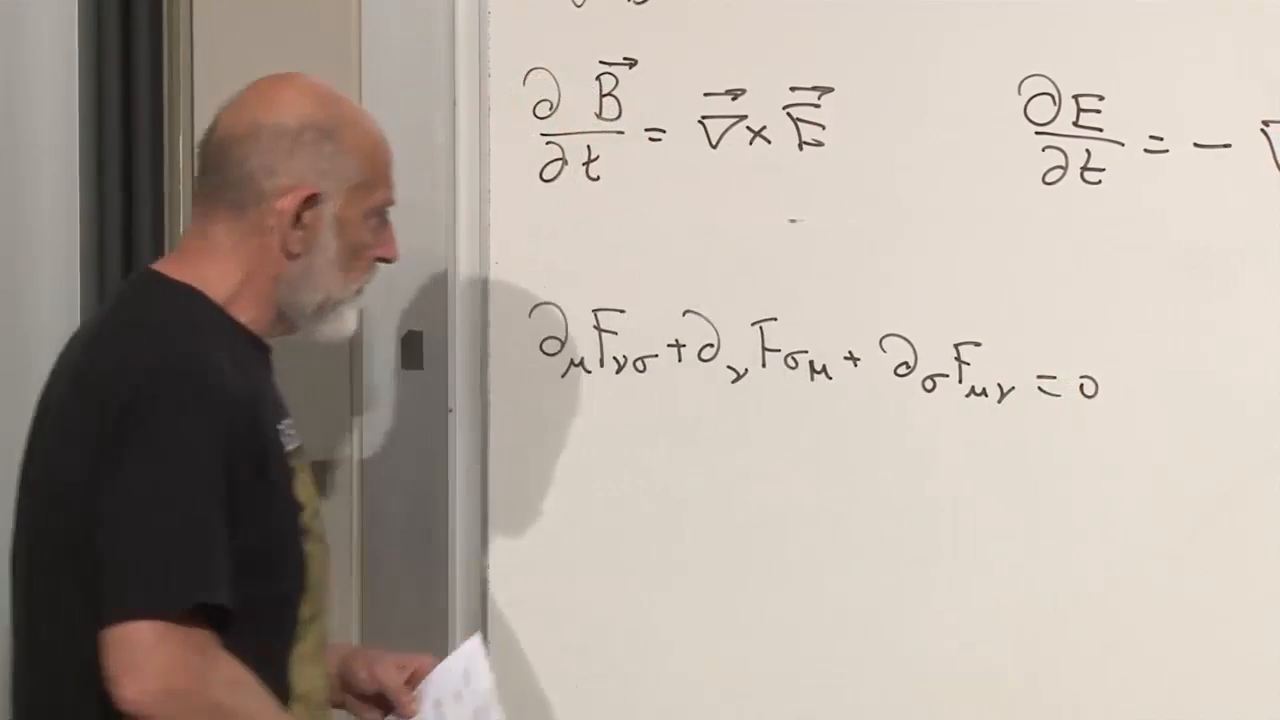
\includegraphics[width=\linewidth]{lecture_09_figure_01.png}
\caption{真空麦克斯韦方程的两族及其协变形式。循环方程是一个恒等式；缩并方程是动力学方程。}
\par\smallskip
\textit{讲义帧：00:03:30。}
\end{figure}

两行之间的区别很重要。方程
\eqref{eq:bianchi-l9}由势\(A_\mu\)的存在而恒等成立：每一项都是二阶导数，各项成对相消。因此它是一个比安基恒等式。相比之下，方程
\eqref{eq:vacuum-maxwell-covariant}是运动方程。改变电磁拉格朗日量，发生改变的就是这一族。

黑板上有一个小观察，它将在本章中发挥两项作用。麦克斯韦方程中的每一个场都以被求导的形式出现。这一事实将约束平面波的相对相位，并且随后会使规范不变性显得自然。

\section{沿\texorpdfstring{\(z\)}{z}轴的平面波}

选择坐标使波沿\(z\)轴传播。这不损失任何一般性；沿其他方向传播的波可以通过旋转坐标轴化为这种形式。设\(k\)为其波数，
\begin{equation}
\lambda=\frac{2\pi}{k},
\end{equation}
并设\(\omega\)为其频率。在施加任何运动方程之前，把全部六个场分量写成具有共同相位
\begin{equation}
\theta=kz-\omega t:
\end{equation}
\begin{align}
E_x(z,t)&=\epsilon_x\sin\theta,
&
B_x(z,t)&=\beta_x\sin\theta,
\nonumber\\
E_y(z,t)&=\epsilon_y\sin\theta,
&
B_y(z,t)&=\beta_y\sin\theta,
\label{eq:plane-wave-ansatz}\\
E_z(z,t)&=\epsilon_z\sin\theta,
&
B_z(z,t)&=\beta_z\sin\theta.
\nonumber
\end{align}
这六个希腊字母是常数振幅。

\begin{figure}[H]
\centering
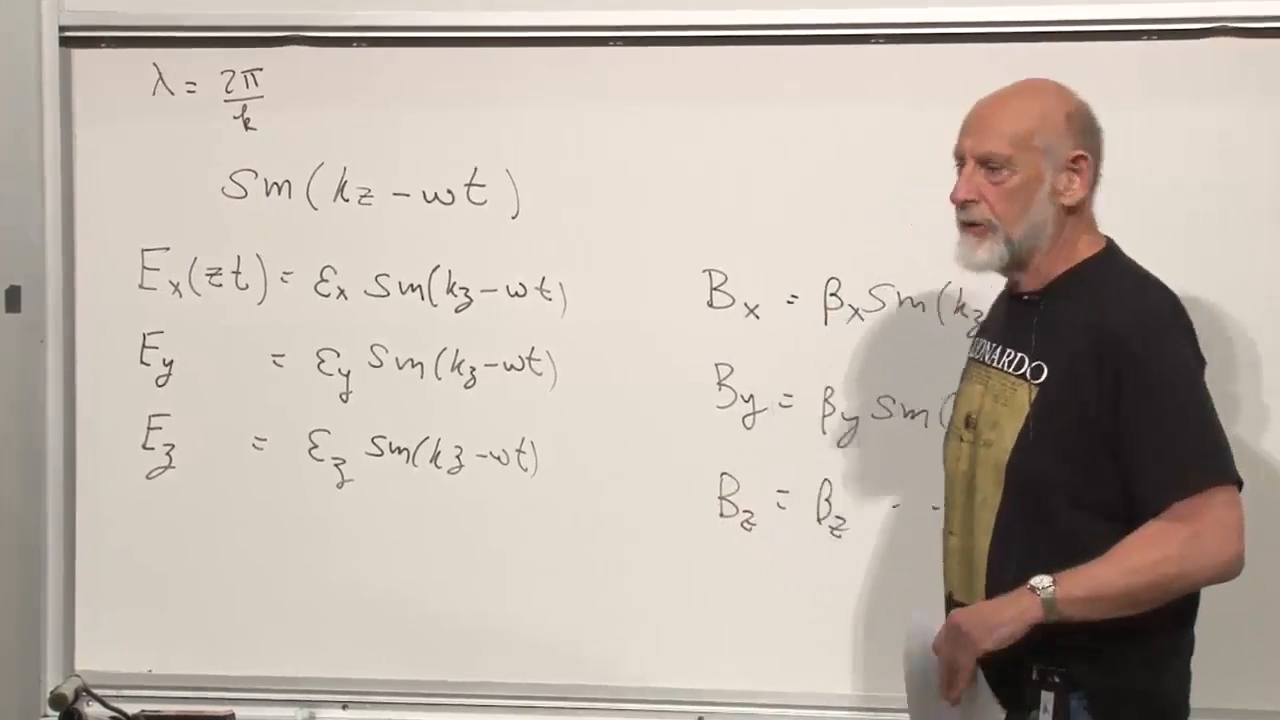
\includegraphics[width=\linewidth]{lecture_09_figure_02.png}
\caption{在麦克斯韦方程剔除被禁止的振幅之前，六分量平面波试探解。}
\par\smallskip
\textit{讲义帧：00:08:45。}
\end{figure}

为什么一开始就让\(\mathbf E\)和\(\mathbf B\)具有相同的正弦依赖？假设一个场带有\(\sin\theta\)，而另一个场带有\(\cos\theta\)。那么旋度方程一侧的时间导数与另一侧的空间导数就会产生不同的三角函数。等式不可能对每一个\(z\)和\(t\)都成立。允许有一个共同的常数相位，但平移\(z\)的原点可以将其消去。因此，这个试探解并不是额外的动力学定律；它只是微分方程所要求的相位关系的最简单代表。

尚未使用任何麦克斯韦方程。我们只是选择了一个方向、一个波长以及一个方便的相位原点。现在方程将决定哪些振幅能够保留下来。

\subsection{散度约束}

因为场只依赖于\(z\)和\(t\)，
\begin{equation}
\nabla\cdot\mathbf E
=
\partial_xE_x+\partial_yE_y+\partial_zE_z
=
\partial_zE_z.
\end{equation}
在真空中这对每一个相位都必须为零，所以
\begin{equation}
\epsilon_z=0.
\label{eq:epsilon-z-zero}
\end{equation}
对磁场作同样的论证给出
\begin{equation}
\beta_z=0.
\label{eq:beta-z-zero}
\end{equation}
两个场都没有沿传播方向的分量。波是横波。

在横向\(xy\)平面内还剩下一个旋转自由度。对\((\epsilon_x,\epsilon_y)\)是一个普通的二维矢量，因此旋转横向坐标轴直到
\begin{equation}
\epsilon_y=0,
\qquad
\epsilon_x\ne0.
\label{eq:polarization-axis}
\end{equation}
这是对线偏振的选择，而不是对物理的限制。

\begin{figure}[H]
\centering
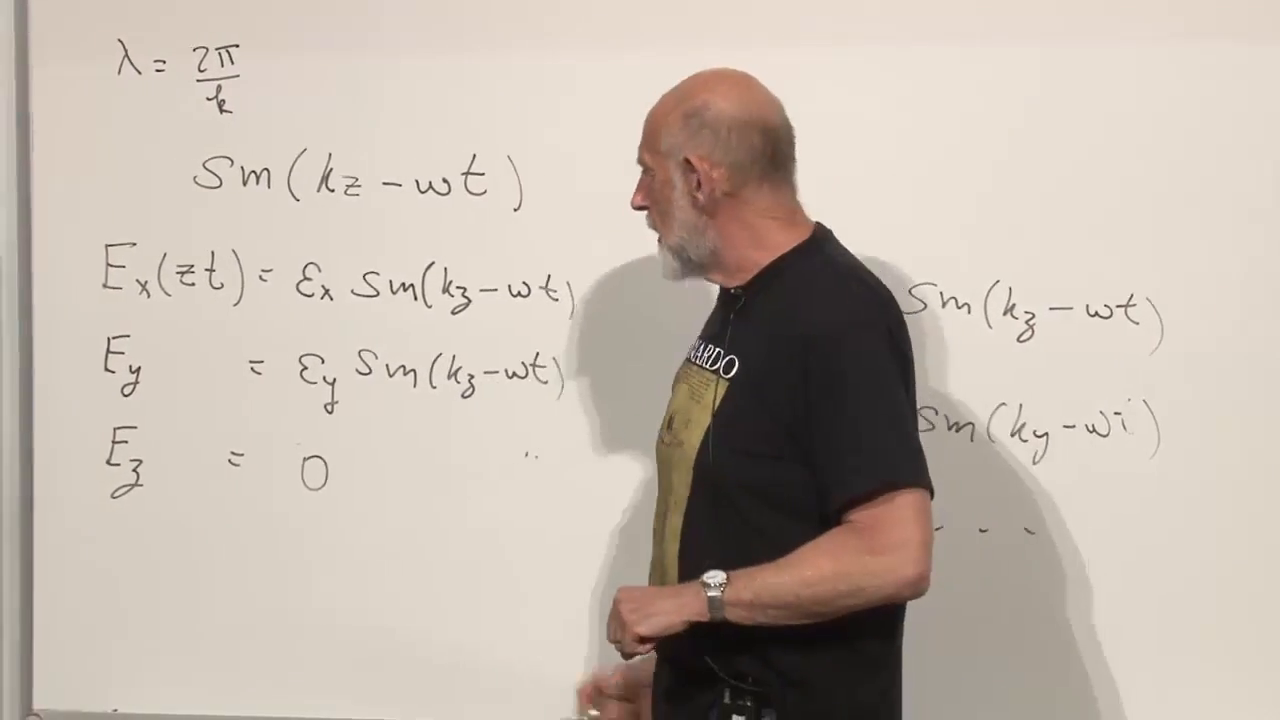
\includegraphics[width=\linewidth]{lecture_09_figure_03.png}
\caption{纵向振幅已经消失，横向电场轴已经选定。}
\par\smallskip
\textit{讲义帧：00:14:30。}
\end{figure}

\subsection{旋度方程}

使用
\(\dot{\mathbf E}=-\nabla\times\mathbf B\)的\(x\)分量。因为场只随\(z\)变化，
\begin{equation}
\dot E_x
=
-\left(\nabla\times\mathbf B\right)_x
=
\partial_zB_y.
\end{equation}
代入试探解给出
\begin{align}
-\omega\epsilon_x\cos\theta
&=
k\beta_y\cos\theta,
\nonumber\\
\beta_y
&=
-\,\epsilon_x\frac{\omega}{k}.
\label{eq:beta-y-epsilon}
\end{align}
同一麦克斯韦方程的\(y\)分量给出
\begin{equation}
\dot E_y
=
-\left(\partial_zB_x\right).
\end{equation}
由我们的偏振选择，左边为零，所以
\begin{equation}
\beta_x=0.
\label{eq:beta-x-zero}
\end{equation}

\begin{figure}[H]
\centering
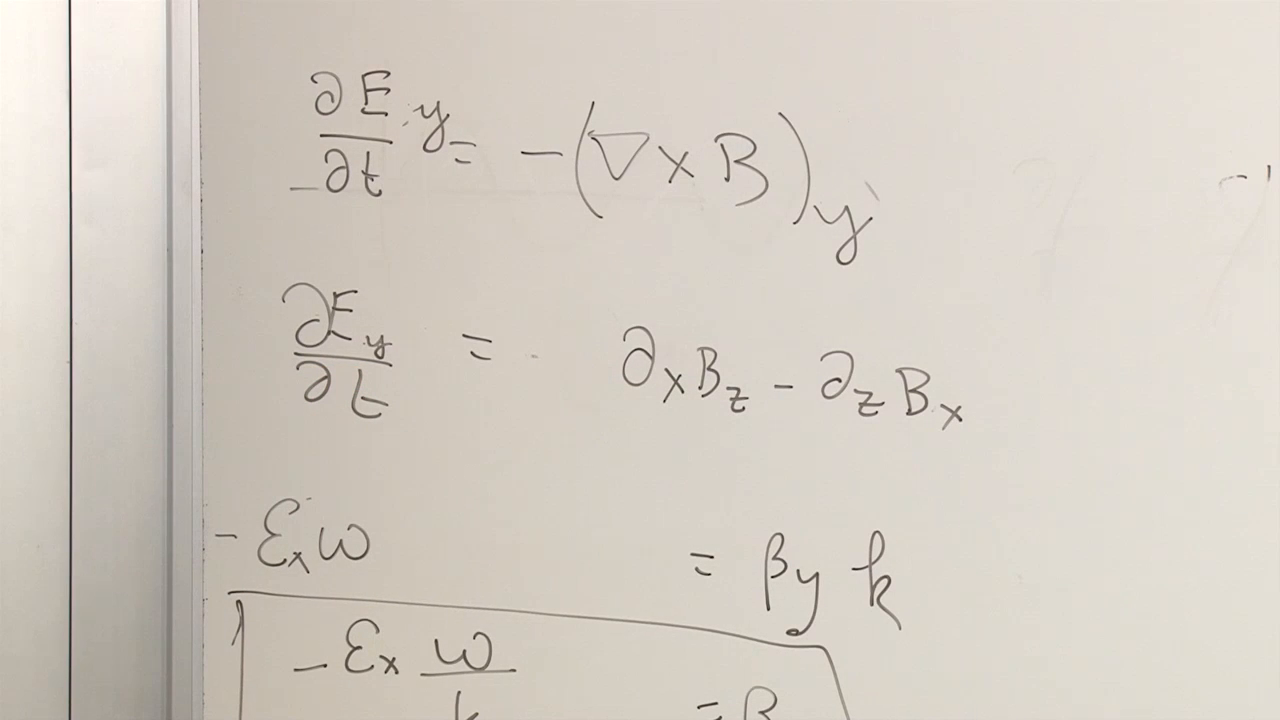
\includegraphics[width=\linewidth]{lecture_09_figure_04.png}
\caption{一个分量旋度计算将\(\epsilon_x\)与\(\beta_y\)联系起来，并消去了剩余的磁振幅。}
\par\smallskip
\textit{讲义画面：00:20:15。}
\end{figure}

因此几何构型是固定的：
\begin{equation}
\mathbf E\parallel\hat{\mathbf x},
\qquad
\mathbf B\parallel\hat{\mathbf y},
\qquad
\mathbf k\parallel\hat{\mathbf z}.
\end{equation}
电场、磁场与传播方向两两相互垂直。

\begin{figure}[H]
\centering
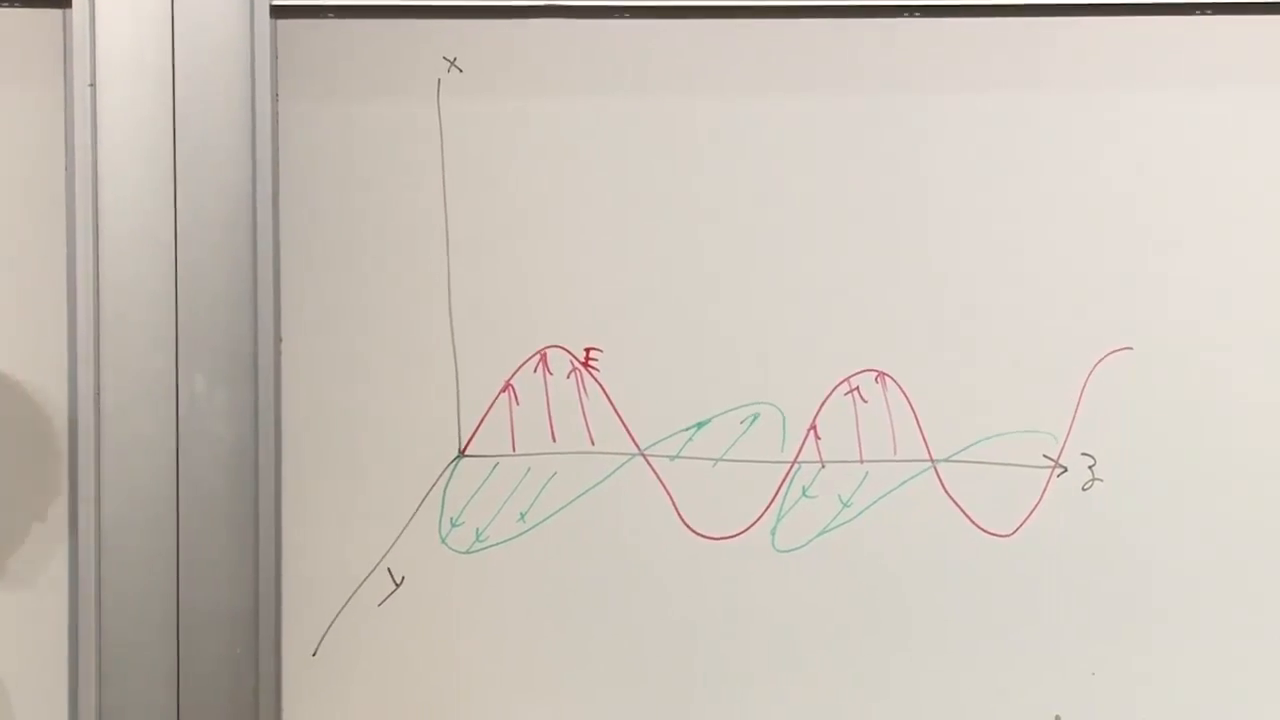
\includegraphics[width=0.94\linewidth]{lecture_09_figure_05.png}
\caption{黑板上画出的横向电场与磁场振荡沿\(z\)轴推进。}
\par\smallskip
\textit{讲义画面：00:23:15。}
\end{figure}

另一个旋度方程给出一个独立的振幅关系。其\(y\)分量为
\begin{equation}
\dot B_y=(\nabla\times\mathbf E)_y=\partial_zE_x,
\end{equation}
因此
\begin{align}
-\omega\beta_y\cos\theta
&=
k\epsilon_x\cos\theta,
\nonumber\\
\epsilon_x
&=
-\,\beta_y\frac{\omega}{k}.
\label{eq:epsilon-beta-y}
\end{align}

\begin{figure}[H]
\centering
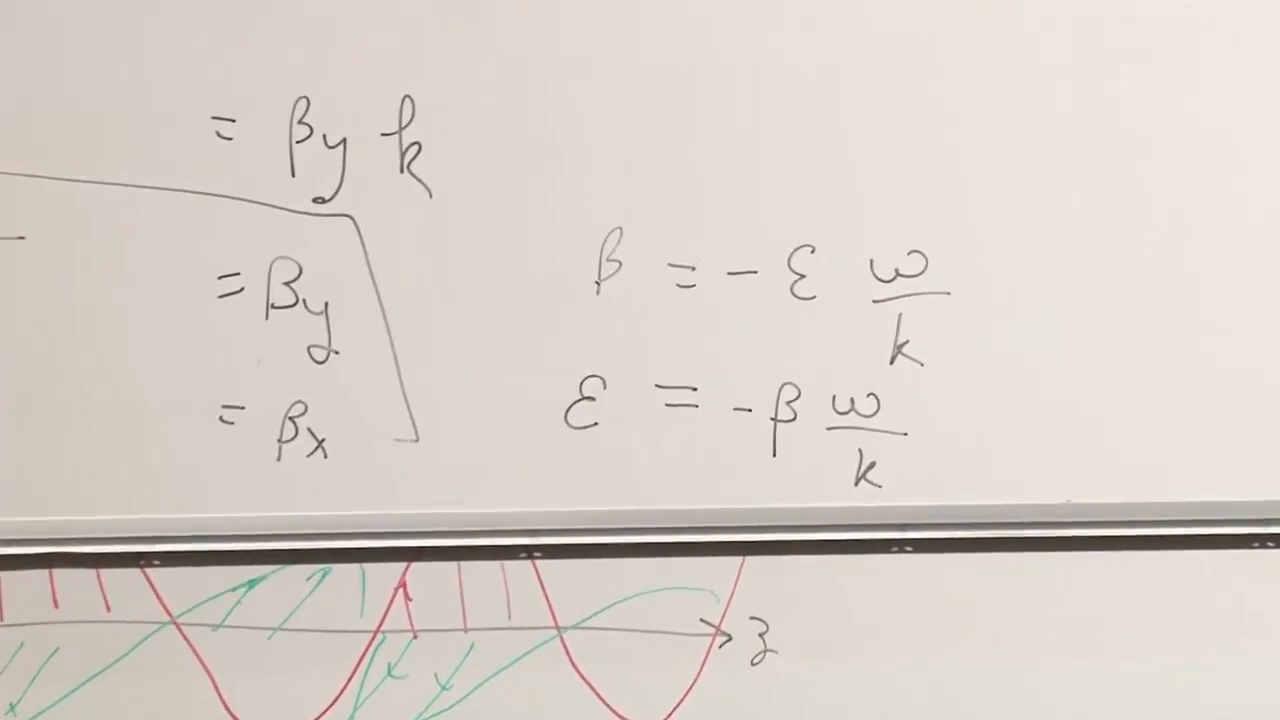
\includegraphics[width=\linewidth]{lecture_09_figure_06.png}
\caption{横向波示意图上方的互反振幅关系。}
\par\smallskip
\textit{讲义画面：00:25:00。}
\end{figure}

将方程\eqref{eq:beta-y-epsilon}与\eqref{eq:epsilon-beta-y}结合，得到色散关系
\begin{equation}
\left(\frac{\omega}{k}\right)^2=1.
\end{equation}
对于沿所选方向传播的正频波，
\begin{equation}
\omega=k
\qquad
(c=1).
\label{eq:omega-k}
\end{equation}
因此公共相位为
\begin{equation}
\theta=k(z-t).
\end{equation}
恢复普通单位后得到
\begin{equation}
\omega=ck,
\qquad
\theta=k(z-ct).
\label{eq:restore-c-wave}
\end{equation}
于是该波形以光速刚性移动。在黑板上所用的单位中，电场振幅与磁场振幅大小相等。它们之间的负号是一种取向约定：它说明所选的\(y\)轴指向哪一侧，而不是说一个场比另一个场滞后四分之一周期。

\begin{figure}[H]
\centering
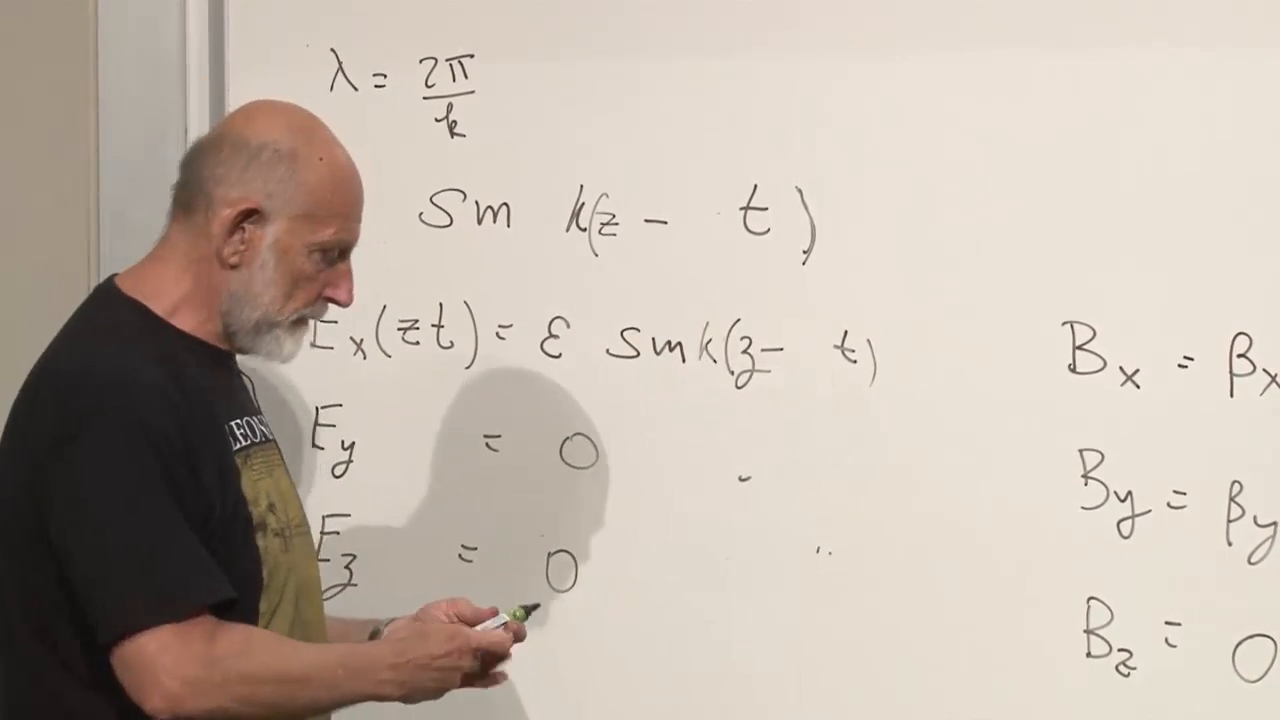
\includegraphics[width=\linewidth]{lecture_09_figure_07.png}
\caption{施加\(\omega=k\)之后得到的最终平面波形式。}
\par\smallskip
\textit{讲义画面：00:26:45。}
\end{figure}

\begin{classroomqa}
\audiencequestion{\(\omega\)与\(k\)难道不具有不同的单位吗？}
\lecturerresponse{在普通单位中确实如此：\(\omega\)是时间的倒数，而\(k\)是长度的倒数。当\(c=1\)时，时间与长度具有相同的单位。恢复\(c\)会把\(\omega=k\)变为\(\omega=ck\)，这正符合量纲分析的要求。\lecturetimestamp{00:25:55}}
\end{classroomqa}

\begin{classroomqa}
\audiencequestion{在平面波中，电场与磁场是否总是同相？}
\lecturerresponse{它们具有相同的相位依赖关系。它们的带符号振幅可以相差一个负号，这可以描述为\(180^\circ\)反转，但对于这个线偏振平面波，麦克斯韦方程组不允许出现\(90^\circ\)正弦--余弦的滞后。圆偏振由横向分量组合而成，需要更谨慎的表述，但它不会改变这一逐分量的麦克斯韦关系。\lecturetimestamp{00:27:31}}
\end{classroomqa}

\begin{classroomqa}
\audiencequestion{如果两个场同时经过零点，能量仍然守恒吗？}
\lecturerresponse{是的。在某个固定点上，能量密度随着波的经过而振荡，但能量是移动了，而不是消失了。在某一时刻占据某一区域的能量，在稍后一刻占据相邻的区域。局域能量输运——由坡印廷通量更完整地表示——使变化的能量密度与守恒相协调。\lecturetimestamp{00:28:15}}
\end{classroomqa}

麦克斯韦方程组是线性的。振幅\(\epsilon_x\)可以大也可以小，\(\beta_y\)由它决定，而解的任意和或差仍是解。因此，沿不同方向传播的波可以叠加。这个简短的计算值得一做：对电磁学的论述不应把电磁波留作一句未经解释的引文。

\begin{classroomqa}
\audiencequestion{推导是否从一开始就假设\(\mathbf E\)与\(\mathbf B\)具有相同的相位？}
\lecturerresponse{公共相位是作为试探解写出的，但它并不是一个独立的物理假设。由于旋度方程的每一侧都对场求导，这些方程会消去非平凡的相对相位。随后，可以通过平移原点来移除一个公共相位移动。\lecturetimestamp{00:29:56}}
\end{classroomqa}

\begin{classroomqa}
\audiencequestion{第二个关系\(\epsilon_x=-\beta_y\omega/k\)是从哪里来的？}
\lecturerresponse{第一个关系来自\(\dot{\mathbf E}=-\nabla\times\mathbf B\)。第二个来自相伴方程\(\dot{\mathbf B}=\nabla\times\mathbf E\)，其中\(\mathbf E\)与\(\mathbf B\)在相同的分量计算中互换。要得到\(\omega^2=k^2\)，两者都是必需的。\lecturetimestamp{00:30:25}}
\end{classroomqa}

\section{为什么仅有微分方程还不够}

现在我们从一个特解转向理论的结构。最小作用量原理正是组织能量守恒、动量守恒以及它们与时空对称性之间关系的东西。人们可以发明出既不具有任何值得称为守恒的能量、也不具有有用对称性原理的微分方程。麦克斯韦方程组则应当从一个拉格朗日量中产生。

只需要产生动力学族：
\begin{equation}
\partial_\mu F^{\mu\nu}=J^\nu.
\label{eq:target-sourced-maxwell}
\end{equation}
Bianchi 族已经由 \(F_{\mu\nu}\) 的定义推出。
用三矢量语言，我们的约定给出
\begin{align}
\nabla\cdot\mathbf E&=\rho,
\label{eq:gauss-source}
\\
\dot{\mathbf E}+\nabla\times\mathbf B&=-\,\mathbf J.
\label{eq:ampere-course-sign}
\end{align}
\eqref{eq:ampere-course-sign} 中的负号很重要。它是 \eqref{eq:target-sourced-maxwell} 在 \eqref{eq:course-f-convention} 下的分量形式，并且将在接近末尾的一次实时符号检验中被重新发现。

\begin{figure}[H]
\centering
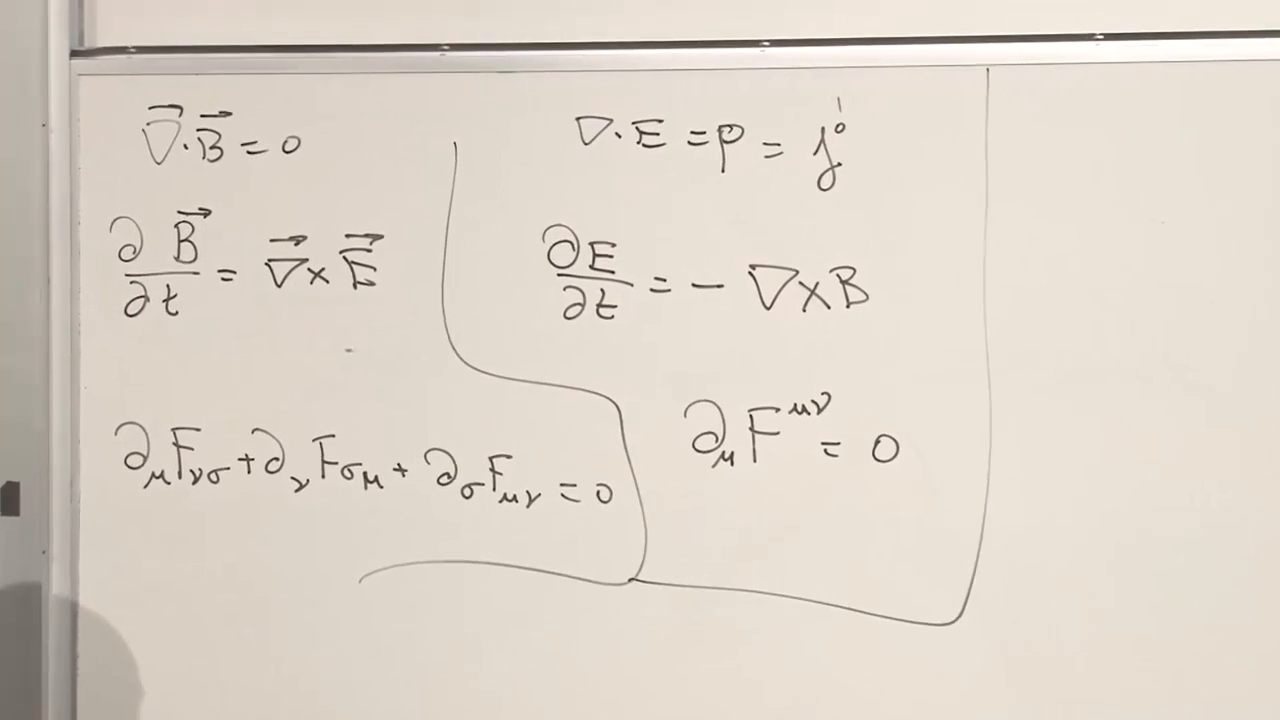
\includegraphics[width=\linewidth]{lecture_09_figure_08.png}
\caption{从波解过渡到作用量原理时的完整 Maxwell 板。}
\par\smallskip
\textit{讲座帧：00:32:45。}
\end{figure}

\section{局域相对论性场论}

第一条原理是局域性。作用量是时空上的一个积分，其被积密度由场及其在同一点的一阶导数构成：
\begin{equation}
S=\int d^4x\,\mathcal L(\phi,\phi_{,\mu}),
\qquad
\phi_{,\mu}\equiv\partial_\mu\phi.
\label{eq:local-action}
\end{equation}
逗号是一种紧凑的导数记号。第二条原理是 Lorentz 不变性：\(\mathcal L\) 必须是一个标量。

\subsection{标量场预演}

在对四矢量进行变分之前，先用一个标量场预演该方法。一个局域 Lorentz 标量可以依赖于势 \(U(\phi)\)，以及两个导数的缩并：
\begin{equation}
\mathcal L_\phi
=
-\frac12\,\partial_\mu\phi\,\partial^\mu\phi-U(\phi).
\label{eq:scalar-lagrangian}
\end{equation}
在 mostly-plus 度规下，
\begin{equation}
\partial_\mu\phi\,\partial^\mu\phi
=
-\dot\phi^{\,2}+|\nabla\phi|^2,
\end{equation}
所以
\begin{equation}
\mathcal L_\phi
=
\frac12\dot\phi^{\,2}
-\frac12|\nabla\phi|^2
-U(\phi).
\end{equation}
升指标的时间导数与降指标的时间导数符号相反；升指标与降指标的空间导数则不然。

\begin{classroomqa}
\audiencequestion{把导数指标放在上面而不是下面，有什么意义吗？}
\lecturerresponse{有。升指标是与逆度规缩并。在号差 \((-+++)\) 下，
\(\partial^0=-\partial_0\)，而
\(\partial^i=\partial_i\)。这就是为什么时间导数项与三个空间项带有相反的符号。
\lecturetimestamp{00:38:02}}
\end{classroomqa}

场的 Euler--Lagrange 方程为
\begin{equation}
\partial_\mu\left(
\frac{\partial\mathcal L}{\partial\phi_{,\mu}}
\right)
=
\frac{\partial\mathcal L}{\partial\phi}.
\label{eq:field-el}
\end{equation}
对于 \eqref{eq:scalar-lagrangian}，
\begin{equation}
\frac{\partial\mathcal L_\phi}{\partial\phi_{,\mu}}
=
-\partial^\mu\phi,
\qquad
\frac{\partial\mathcal L_\phi}{\partial\phi}
=
-U'(\phi),
\end{equation}
因此
\begin{equation}
\Box\phi=U'(\phi),
\qquad
\Box\equiv\partial_\mu\partial^\mu.
\end{equation}
等价地，
\begin{equation}
\ddot\phi-\nabla^2\phi=-U'(\phi).
\label{eq:scalar-wave}
\end{equation}
在黑板上，只写出 \(x\) 导数，而 \(y\) 和 \(z\) 项被隐含。结果就是熟悉的、带有来自势的力的波动方程。

\begin{figure}[H]
\centering
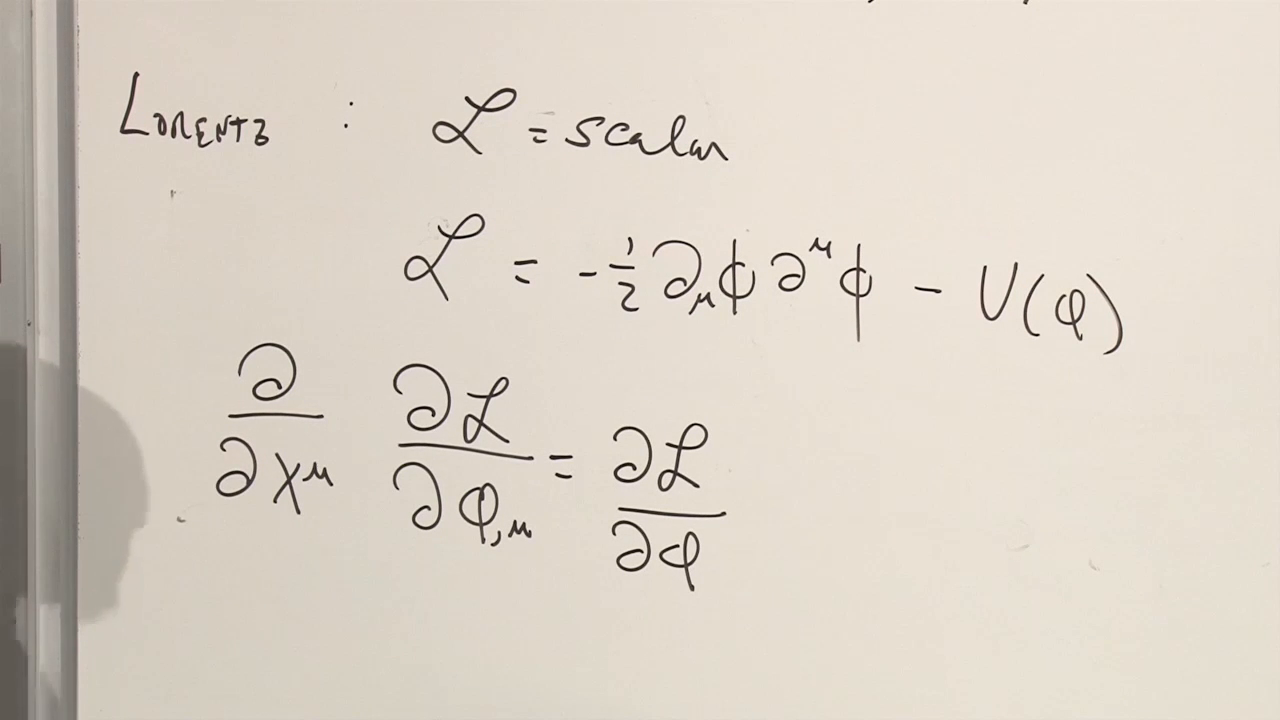
\includegraphics[width=\linewidth]{lecture_09_figure_09.png}
\caption{局域性、标量 Lorentz 不变拉格朗日量，以及场论 Euler--Lagrange 方程。}
\par\smallskip
\textit{讲座帧：00:41:00。}
\end{figure}

电磁计算是同样的变分过程，只是有四个场和更多的指标。

\section{规范不变性选出 Maxwell 标量}

加入第三条原理：规范不变性。暂时设 \(J^\mu=0\)，并考虑自由场。规范变换是
\begin{equation}
A_\mu\longrightarrow A_\mu+\partial_\mu\chi.
\label{eq:gauge-transform}
\end{equation}
场张量不变，因为混合二阶导数可交换：
\begin{align}
F_{\mu\nu}
&\longrightarrow
F_{\mu\nu}
+\partial_\mu\partial_\nu\chi
-\partial_\nu\partial_\mu\chi
\nonumber\\
&=F_{\mu\nu}.
\end{align}

仅凭 Lorentz 不变性会允许标量
\begin{equation}
A_\mu A^\mu.
\end{equation}
然而它在 Maxwell 理论中被禁止，因为它在 \eqref{eq:gauge-transform} 下会改变。这个表达式中的指标标记场分量；它们不是导数。导数用逗号表示，如 \(A_{\nu,\mu}=\partial_\mu A_\nu\)。

\begin{figure}[H]
\centering
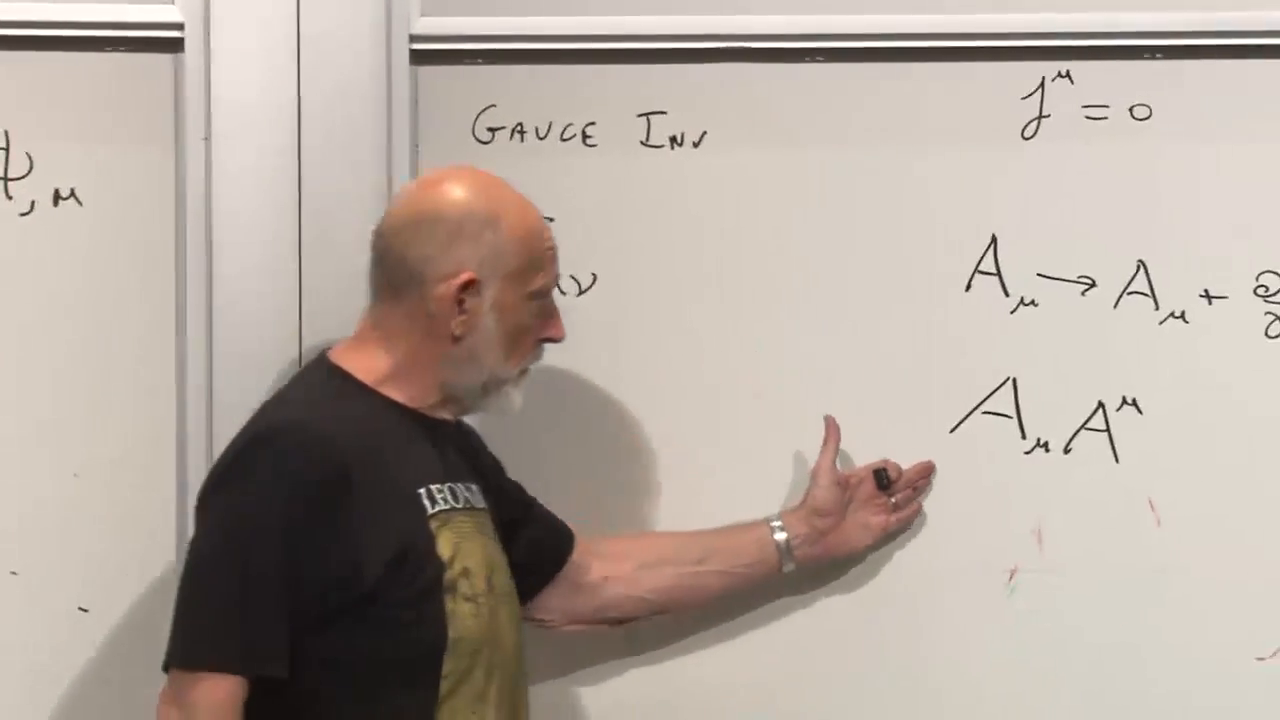
\includegraphics[width=\linewidth]{lecture_09_figure_10.png}
\caption{规范变换以及 Lorentz 标量 \(A_\mu A^\mu\)，后者因不是规范不变的而被拒绝。}
\par\smallskip
\textit{讲座帧：00:43:40。}
\end{figure}

因此我们应当用 \(F_{\mu\nu}\) 来构造自由拉格朗日量。线性迹不成立：
\begin{equation}
F^\mu{}_\mu=0.
\end{equation}
反对称性迫使每个对角分量都为零：
\begin{equation}
F_{00}=F_{11}=F_{22}=F_{33}=0.
\end{equation}
升指标可能会改变一个符号，但它不能把零变成别的东西。

\begin{figure}[H]
\centering
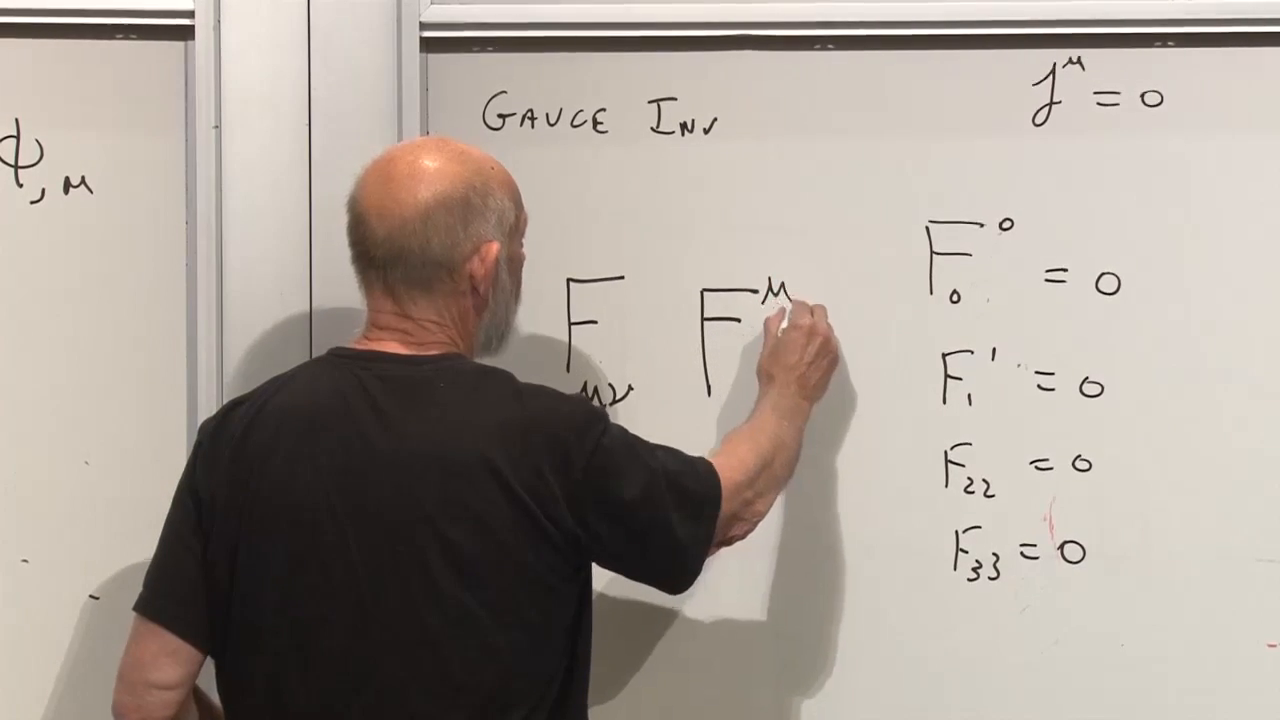
\includegraphics[width=\linewidth]{lecture_09_figure_11.png}
\caption{尝试的线性迹以及反对称场张量的零对角元。}
\par\smallskip
\textit{讲座帧：00:47:00。}
\end{figure}

第一个非零 Lorentz 标量是二次的：
\begin{equation}
F_{\mu\nu}F^{\mu\nu}.
\label{eq:f2-scalar}
\end{equation}
让我们展开这个缩并，而不是直接引用它。混合分量包含电场。升高它们的时间指标会贡献一个负号，并且两种次序 \(0i\) 和 \(i0\) 都会出现：
\begin{equation}
\sum_i\left(F_{0i}F^{0i}+F_{i0}F^{i0}\right)
=-2E^2.
\end{equation}
纯空间分量包含磁场。升高空间指标不改变符号，并且两种次序同样都会出现：
\begin{equation}
\sum_{i<j}\left(F_{ij}F^{ij}+F_{ji}F^{ji}\right)
=2B^2.
\end{equation}
因此
\begin{equation}
F_{\mu\nu}F^{\mu\nu}=2(B^2-E^2),
\qquad
-F_{\mu\nu}F^{\mu\nu}=2(E^2-B^2).
\label{eq:f2-eb}
\end{equation}

\begin{figure}[H]
\centering
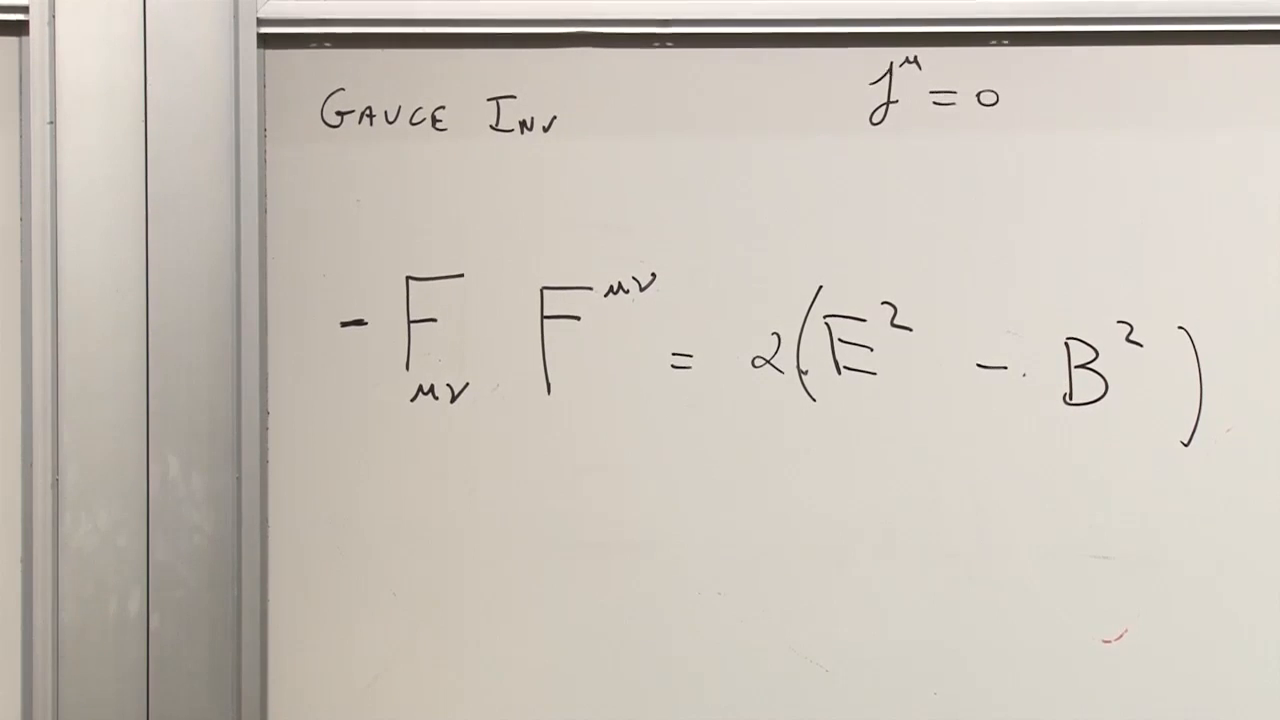
\includegraphics[width=\linewidth]{lecture_09_figure_12.png}
\caption{用电场和磁场大小表示的完整缩并。}
\par\smallskip
\textit{讲座帧：00:51:00。}
\end{figure}

\begin{classroomqa}
\audiencequestion{\(F_{00}\) 也是零吗？}
\lecturerresponse{是。反对称张量的每个对角分量都为零，包括 \(F_{00}\)。只有编码 \(\mathbf E\) 的非对角混合分量，以及编码 \(\mathbf B\) 的非对角空间分量，才有贡献。
\lecturetimestamp{00:51:36}}
\end{classroomqa}

常规归一化是
\begin{equation}
\boxed{
\mathcal L_{\mathrm{EM}}
=
-\frac14F_{\mu\nu}F^{\mu\nu}
}
\label{eq:maxwell-lagrangian}
\end{equation}
或
\begin{equation}
\mathcal L_{\mathrm{EM}}
=
\frac12(E^2-B^2).
\label{eq:maxwell-lagrangian-eb}
\end{equation}
负号使电场项获得熟悉的正确符号。因子\(1/4\)补偿了每一对反对称组合的两次出现，并留下常规因子\(1/2\)。将整个自由作用量乘以一个非零常数不会改变其无源方程，但这一归一化才是与标准源耦合相匹配的归一化。

\section{变分自由电磁场}

独立场为
\begin{equation}
A_0,\qquad A_x,\qquad A_y,\qquad A_z.
\end{equation}
对每个分量\(A_\nu\)，欧拉--拉格朗日方程为
\begin{equation}
\partial_\mu\left(
\frac{\partial\mathcal L}{\partial A_{\nu,\mu}}
\right)
=
\frac{\partial\mathcal L}{\partial A_\nu},
\qquad
A_{\nu,\mu}\equiv\partial_\mu A_\nu.
\label{eq:vector-el-comma}
\end{equation}
逗号记号中的位置值得慢慢读：第一个指标标记\(A\)的哪个分量是场；第二个指标标记求导的坐标。

在此记号下，
\begin{equation}
F_{\mu\nu}
=
A_{\nu,\mu}-A_{\mu,\nu}.
\label{eq:f-comma-consistent}
\end{equation}
这正是\eqref{eq:course-f-convention}。以相反的口头顺序书写逗号指标会改变一个中间负号，这就是为什么分量计算是有用的。

\begin{figure}[H]
\centering
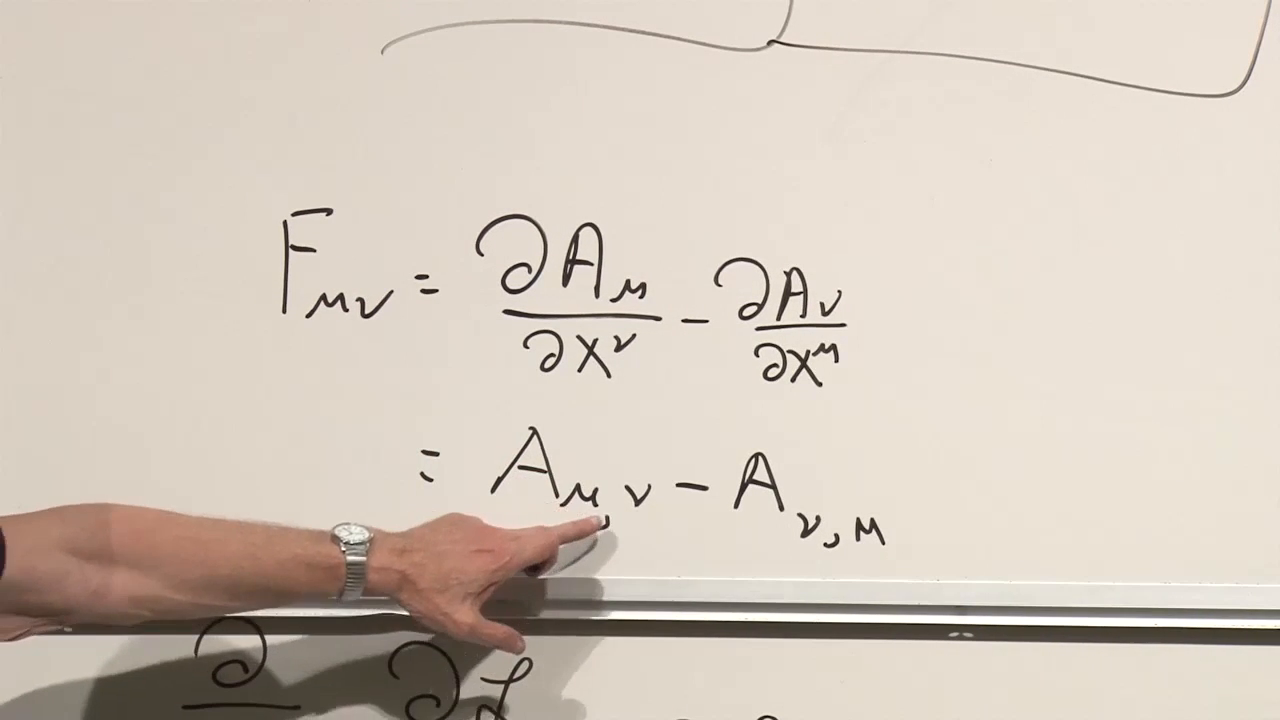
\includegraphics[width=\linewidth]{lecture_09_figure_13.png}
\caption{在四个势分量被确定为独立场之后，用逗号记号表示的场张量。}
\par\smallskip
\textit{授课帧：00:55:30。}
\end{figure}

\begin{figure}[H]
\centering
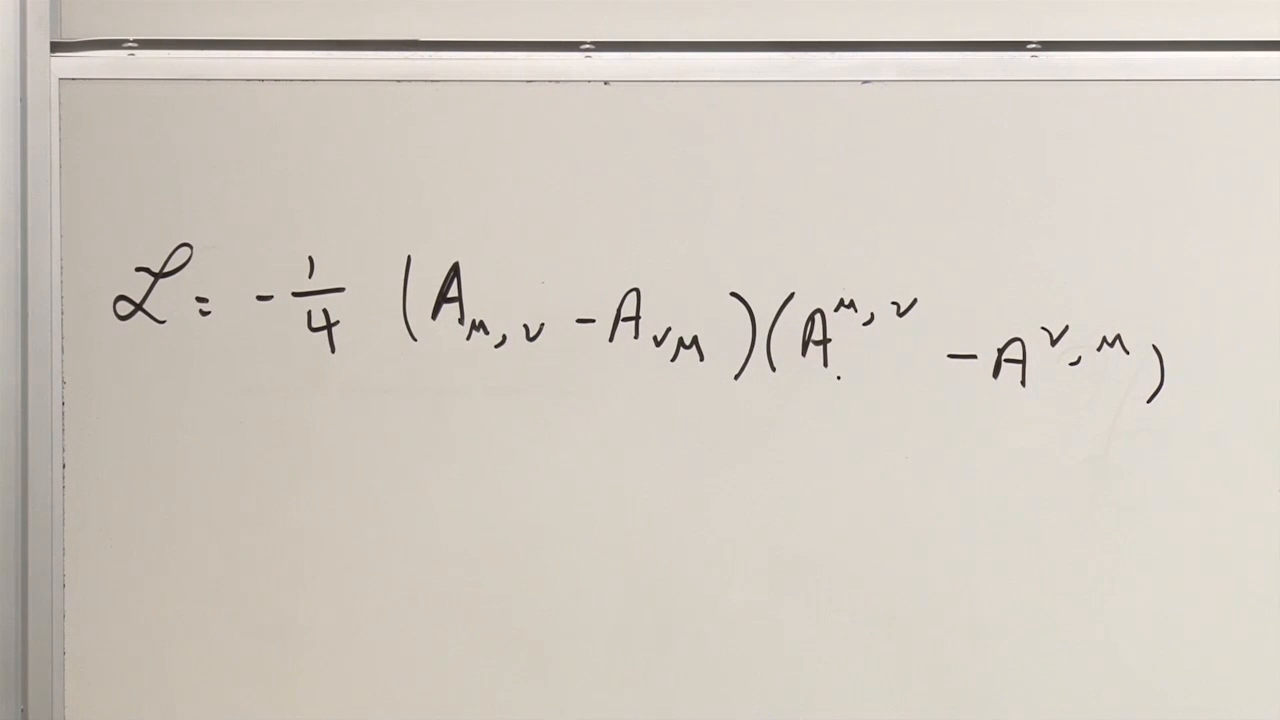
\includegraphics[width=\linewidth]{lecture_09_figure_14.png}
\caption{用矢量势的导数显式写出的麦克斯韦拉格朗日量。}
\par\smallskip
\textit{授课帧：00:56:45。}
\end{figure}

\subsection{一个代表性导数}

选取导数\(A_{x,y}=\partial_yA_x\)。完整求和中\(xy\)与\(yx\)两项贡献
\begin{align}
\mathcal L_{\mathrm{EM}}
&\supset
-\frac14\left(F_{xy}F^{xy}+F_{yx}F^{yx}\right)
\nonumber\\
&=
-\frac12F_{xy}^2
\nonumber\\
&=
-\frac12\left(A_{x,y}-A_{y,x}\right)^2.
\label{eq:isolated-xy-piece}
\end{align}
最后一个等号是安全的，因为平方后符号消失：\(A_{x,y}-A_{y,x}=F_{yx}=-F_{xy}\)。

\begin{figure}[H]
\centering
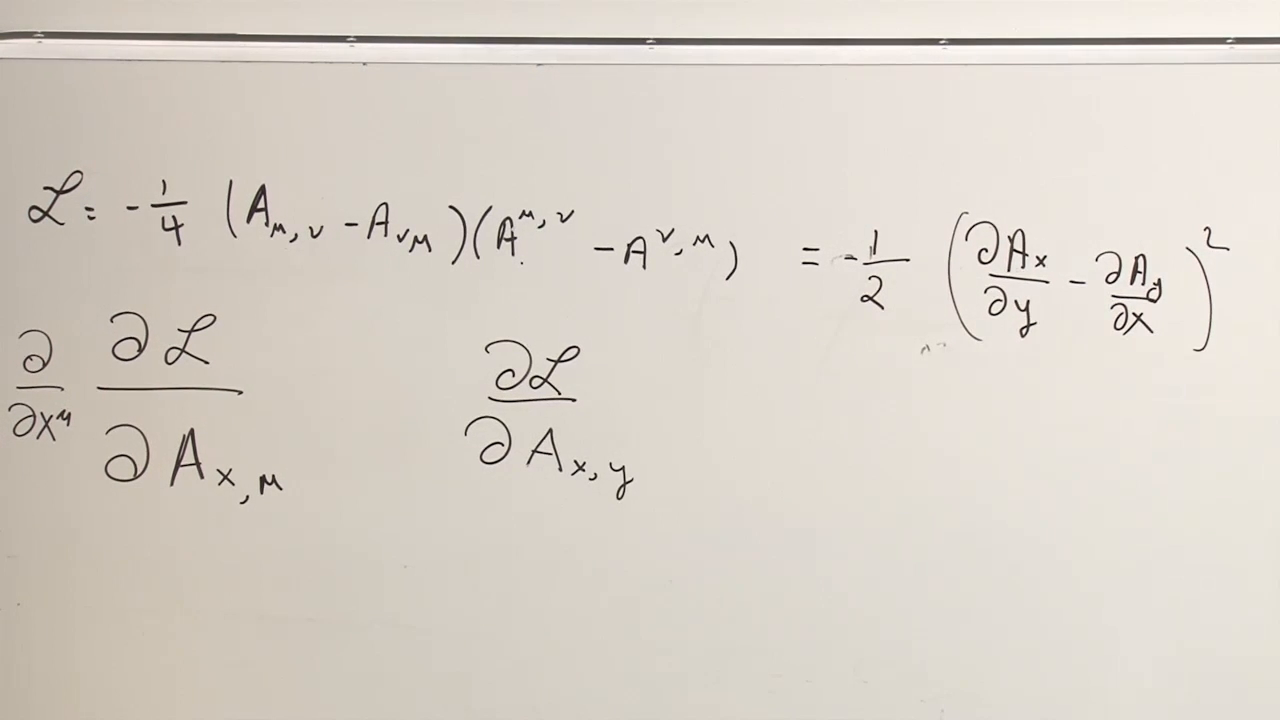
\includegraphics[width=\linewidth]{lecture_09_figure_15.png}
\caption{代表性的\(A_{x,y}\)导数与分离出的反对称平方。}
\par\smallskip
\textit{授课帧：01:00:45。}
\end{figure}

求导：
\begin{align}
\frac{\partial\mathcal L_{\mathrm{EM}}}
{\partial A_{x,y}}
&=
-\left(A_{x,y}-A_{y,x}\right)
\nonumber\\
&=
F_{xy}.
\label{eq:component-variation}
\end{align}
板书用负号总结这一点，该负号附着于指标顺序遵循板书求导顺序的张量。采用课程统一定义\eqref{eq:course-f-convention}，不变量形式的陈述为
\begin{equation}
\frac{\partial\mathcal L_{\mathrm{EM}}}
{\partial(\partial_\mu A_\nu)}
=
-F^{\mu\nu}.
\label{eq:maxwell-canonical-derivative}
\end{equation}
对于例子\(\partial_yA_x\)，这给出
\(-F^{yx}=F^{xy}\)，正是
\eqref{eq:component-variation}。因此表面上的符号差异只是指标顺序的记账问题。

\begin{figure}[H]
\centering
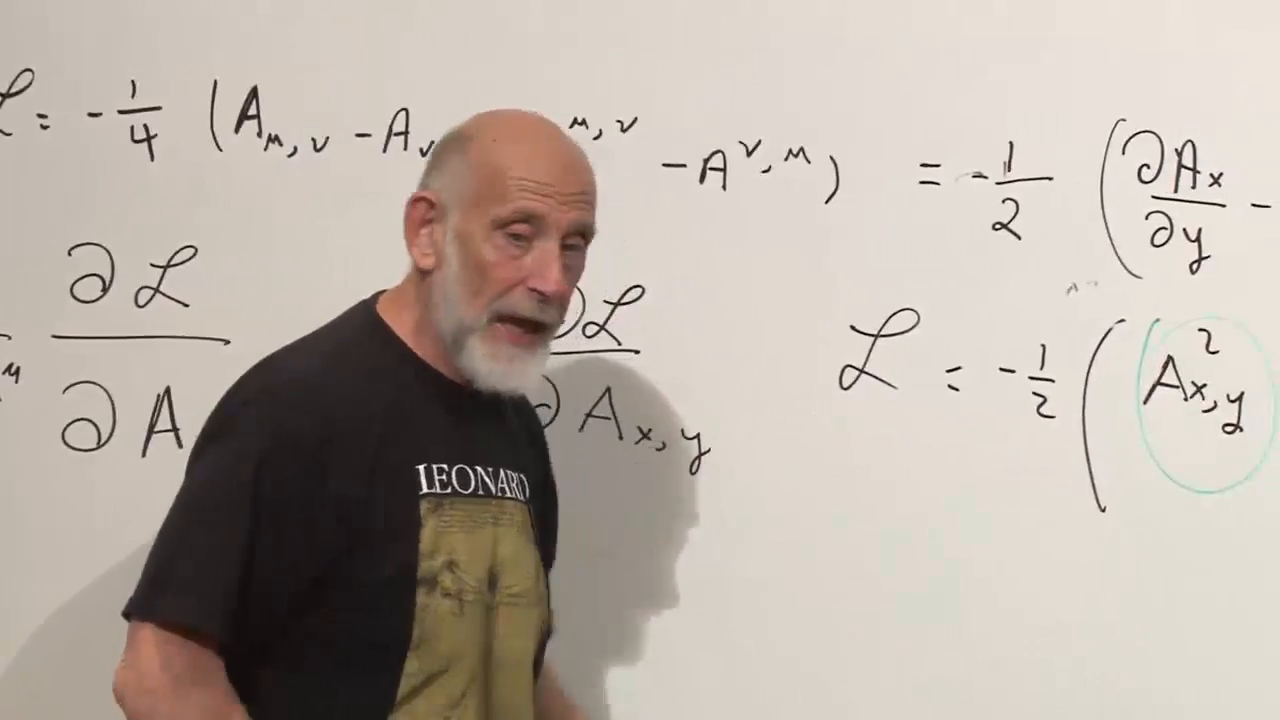
\includegraphics[width=\linewidth]{lecture_09_figure_16.png}
\caption{在对势的一个导数求导之前，展开所选平方项。}
\par\smallskip
\textit{授课帧：01:03:00。}
\end{figure}

\begin{classroomqa}
\audiencequestion{分量导数中的因子\(1/2\)到哪里去了？}
\lecturerresponse{对平方项求导给出一个因子二，它抵消了\(1/2\)：
\[
\frac{d}{dx}\left[-\frac12x^2\right]=-x.
\]
先前从\(1/4\)到\(1/2\)的变化来自两个有序张量分量\(xy\)和\(yx\)。\lecturetimestamp{01:03:29}}
\end{classroomqa}

真空拉格朗日量中没有未求导的势：
\begin{equation}
\frac{\partial\mathcal L_{\mathrm{EM}}}{\partial A_\nu}=0.
\end{equation}
代入\eqref{eq:vector-el-comma}给出
\begin{equation}
-\partial_\mu F^{\mu\nu}=0,
\end{equation}
或等价地
\begin{equation}
\boxed{\partial_\mu F^{\mu\nu}=0.}
\label{eq:free-maxwell-from-action}
\end{equation}

\begin{figure}[H]
\centering
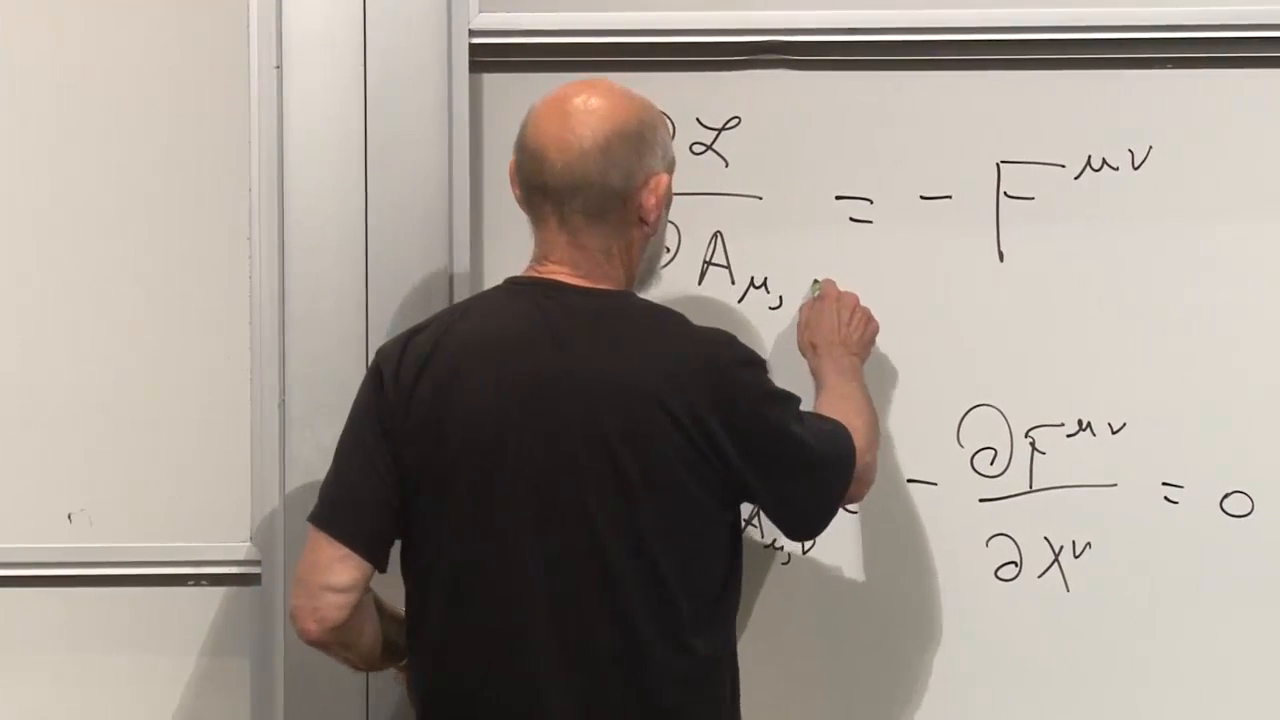
\includegraphics[width=\linewidth]{lecture_09_figure_17.png}
\caption{将分量结果推广并代入欧拉--拉格朗日方程。}
\par\smallskip
\textit{授课帧：01:09:00。}
\end{figure}

通过变分整个作用量可以更干净地得到同一结论：
\begin{align}
\delta S_{\mathrm{EM}}
&=
-\frac12\int d^4x\,
F^{\mu\nu}
\left(\partial_\mu\delta A_\nu
-\partial_\nu\delta A_\mu\right)
\nonumber\\
&=
-\int d^4x\,F^{\mu\nu}\partial_\mu\delta A_\nu
\nonumber\\
&=
\int d^4x\,
\left(\partial_\mu F^{\mu\nu}\right)\delta A_\nu,
\label{eq:global-maxwell-variation}
\end{align}
其中边界项被丢弃。反对称性合并了第一行中的两项。由于\(\delta A_\nu\)是任意的，
\eqref{eq:free-maxwell-from-action}随之成立。

\begin{classroomqa}
\audiencequestion{分离出的平方项是否假设磁场只指向\(z\)方向？}
\lecturerresponse{不。它只是从完整求和中取出用于检查的一项；其后应有一个省略号。其余空间对给出其他磁场分量，而时间--空间对给出电场分量。\lecturetimestamp{01:08:05}}
\end{classroomqa}

\begin{classroomqa}
\audiencequestion{选择一个时间指标而不是两个空间指标会改变结果吗？}
\lecturerresponse{它给出相同的一般导数，度规符号由指标升降处理。两个空间指标选出一个磁场分量；一个时间指标和一个空间指标选出一个电场分量。反对称公式
\eqref{eq:maxwell-canonical-derivative}涵盖两者。
\lecturetimestamp{01:08:46}}
\end{classroomqa}

\begin{classroomqa}
\audiencequestion{我们仍然假设\(J^\mu=0\)吗？}
\lecturerresponse{仅在这一自由场推导中如此。电流被暂时设为零，以便能够识别规范不变的动能项。现在我们恢复它，并问哪一额外项产生麦克斯韦方程右边的项。\lecturetimestamp{01:09:41}}
\end{classroomqa}

这些代数并不难，但必须亲手推一遍，而不能只是看着。顺着指标链走一遍并不能使它牢固；必须亲手把这条链重新推出来才行。

\section{守恒的四维电流}

源就是四维电流
\begin{equation}
J^\mu=(\rho,\mathbf J).
\end{equation}
它的时间分量是电荷密度，空间分量是穿过三个相互垂直的窗口的电荷通量。等价地，对于一个小的固定盒子，
\begin{equation}
\frac{\partial\rho}{\partial t}
+\nabla\cdot\mathbf J=0.
\label{eq:continuity-vector-l9}
\end{equation}
盒内的电荷只能通过其边界流出而减少。用协变记号表示，
\begin{equation}
\boxed{\partial_\mu J^\mu=0.}
\label{eq:continuity-covariant-l9}
\end{equation}

\begin{figure}[H]
\centering
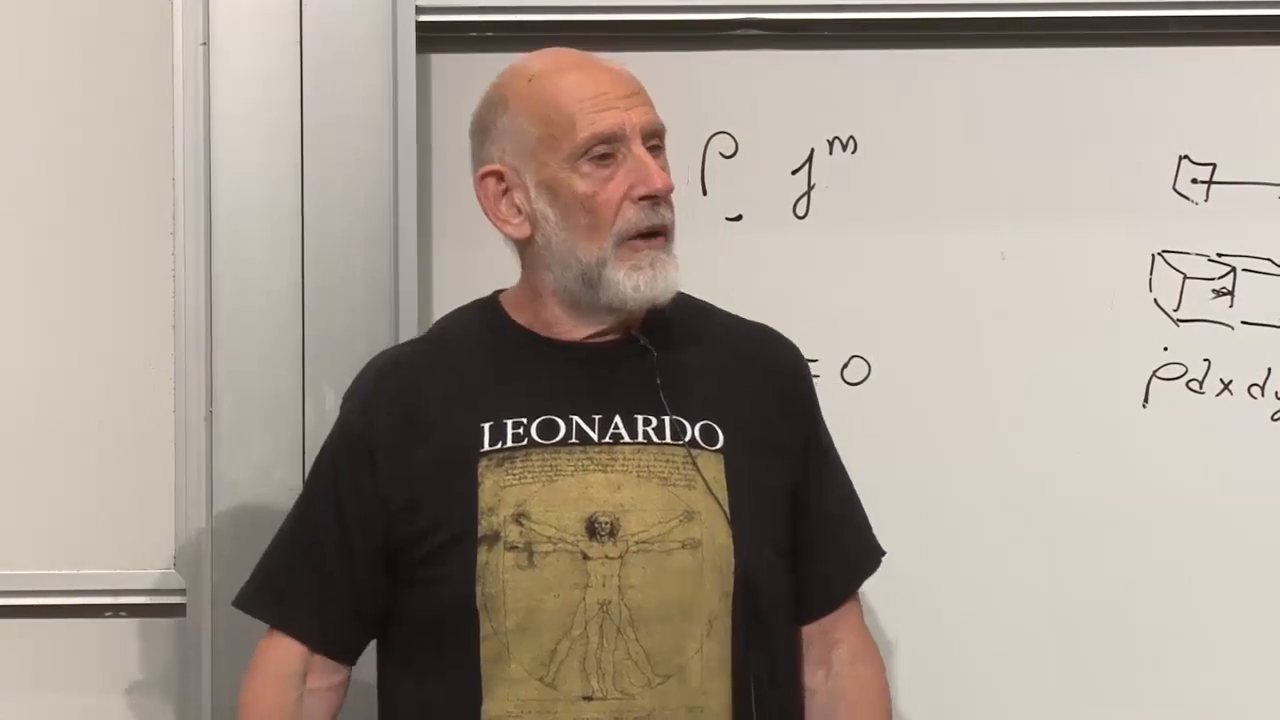
\includegraphics[width=\linewidth]{lecture_09_figure_18.png}
\caption{在引入源耦合之前回顾的电荷密度、空间电流以及小盒子的解释。}
\par\smallskip
\textit{讲课画面：01:14:45。}
\end{figure}

\section{源耦合与规范不变性}

同时关于电流和势为线性的最简单的局域洛伦兹标量是
\begin{equation}
S_{\mathrm{int}}
=
-\int d^4x\,J^\mu A_\mu.
\label{eq:interaction-action}
\end{equation}
整体符号是约定俗成的。课上开玩笑说，历史上对电荷符号的选择最终可以归咎于本杰明·富兰克林；真正的要点是，必须在所有地方使用同一个自洽的符号约定。

乍看之下，\eqref{eq:interaction-action} 并不显得规范不变。在 \eqref{eq:gauge-transform} 下，
\begin{equation}
\delta_\chi S_{\mathrm{int}}
=
-\int d^4x\,J^\mu\partial_\mu\chi.
\label{eq:gauge-variation-interaction}
\end{equation}

\begin{figure}[H]
\centering
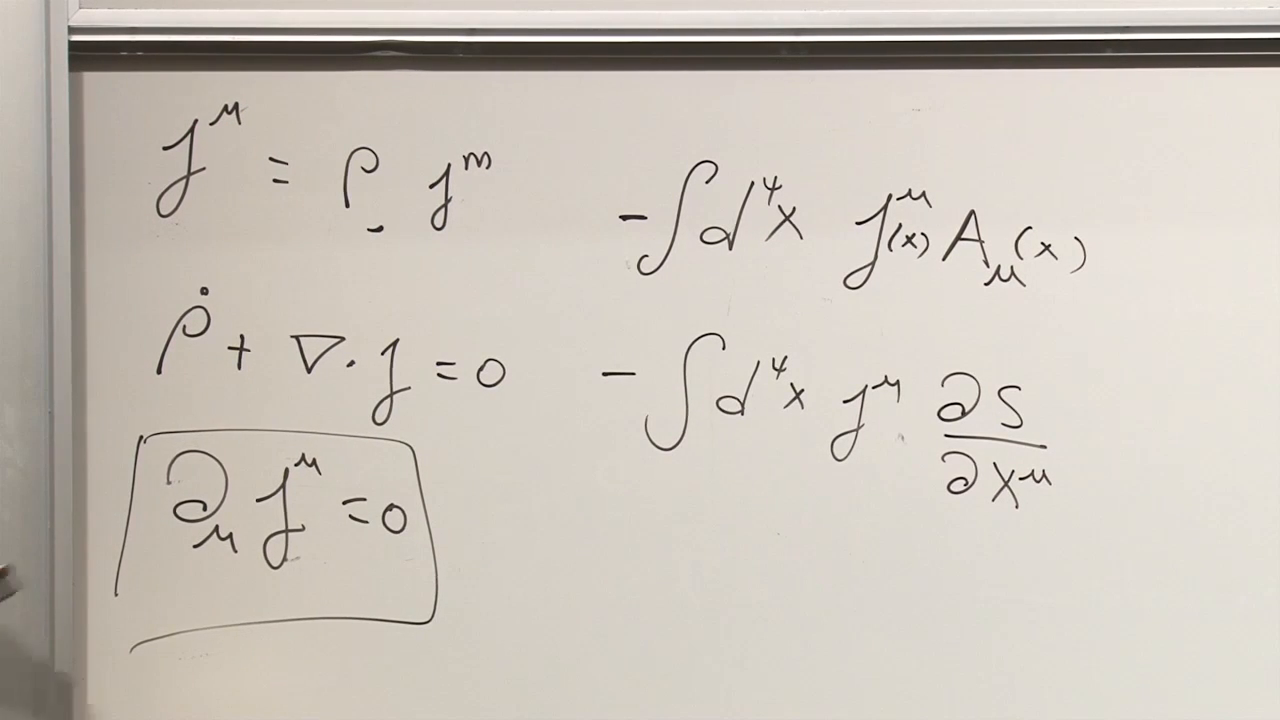
\includegraphics[width=\linewidth]{lecture_09_figure_19.png}
\caption{相互作用作用量及其在
\(A_\mu\mapsto A_\mu+\partial_\mu\chi\) 下的变分。}
\par\smallskip
\textit{讲课画面：01:16:45。}
\end{figure}

为了从初等层面看清其机制，把缩并展开：
\begin{equation}
J^\mu\partial_\mu\chi
=
J^0\partial_0\chi
+J^1\partial_1\chi
+J^2\partial_2\chi
+J^3\partial_3\chi.
\end{equation}
假设电流被限制在一个大的实验室范围内，或者衰减得足够快，以致在边界处为零。对每一项分部积分。例如，对于第一个空间坐标，
\begin{align}
-\int d^4x\,J^1\partial_1\chi
&=
-\int dt\,dx^2\,dx^3
\left[J^1\chi\right]_{x^1=-\infty}^{x^1=+\infty}
\nonumber\\
&\quad
+\int d^4x\,\chi\,\partial_1J^1
\nonumber\\
&=
\int d^4x\,\chi\,\partial_1J^1.
\end{align}
同样的操作适用于时间项和另外两个空间项。

\begin{figure}[H]
\centering
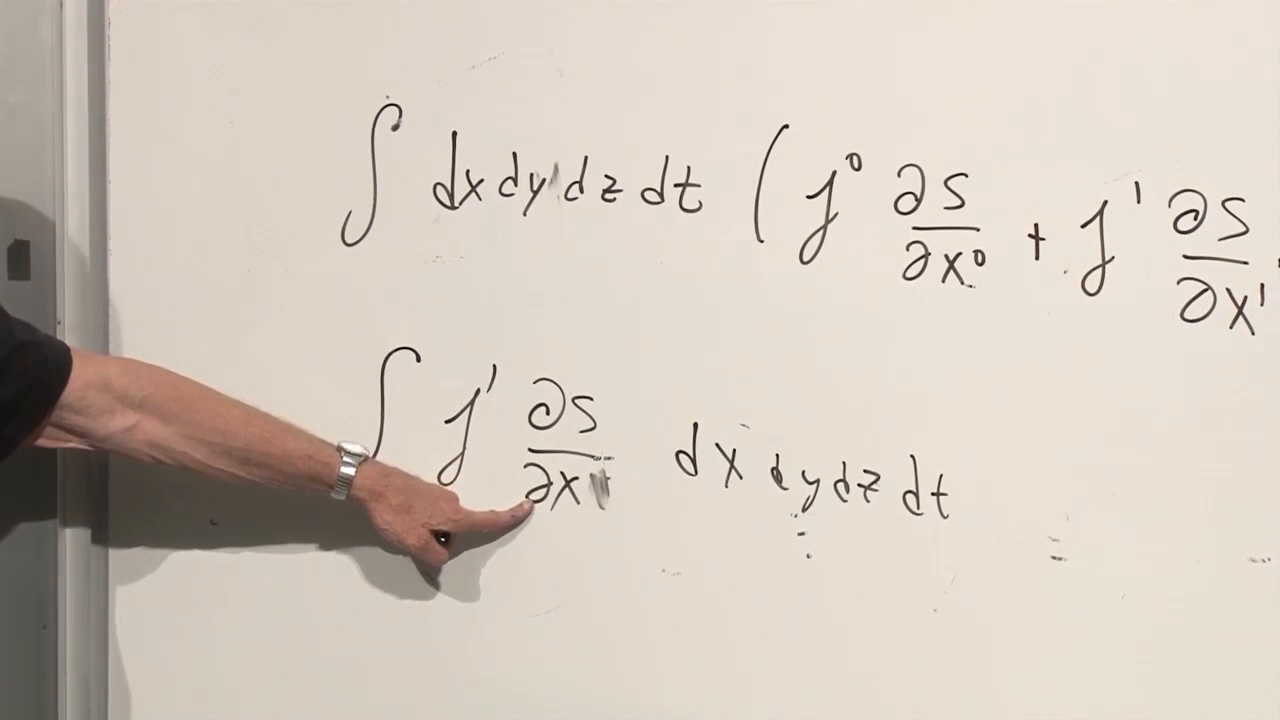
\includegraphics[width=\linewidth]{lecture_09_figure_20.png}
\caption{分部积分之前展开的四个规范变分项。}
\par\smallskip
\textit{讲课画面：01:19:15。}
\end{figure}

\begin{figure}[H]
\centering
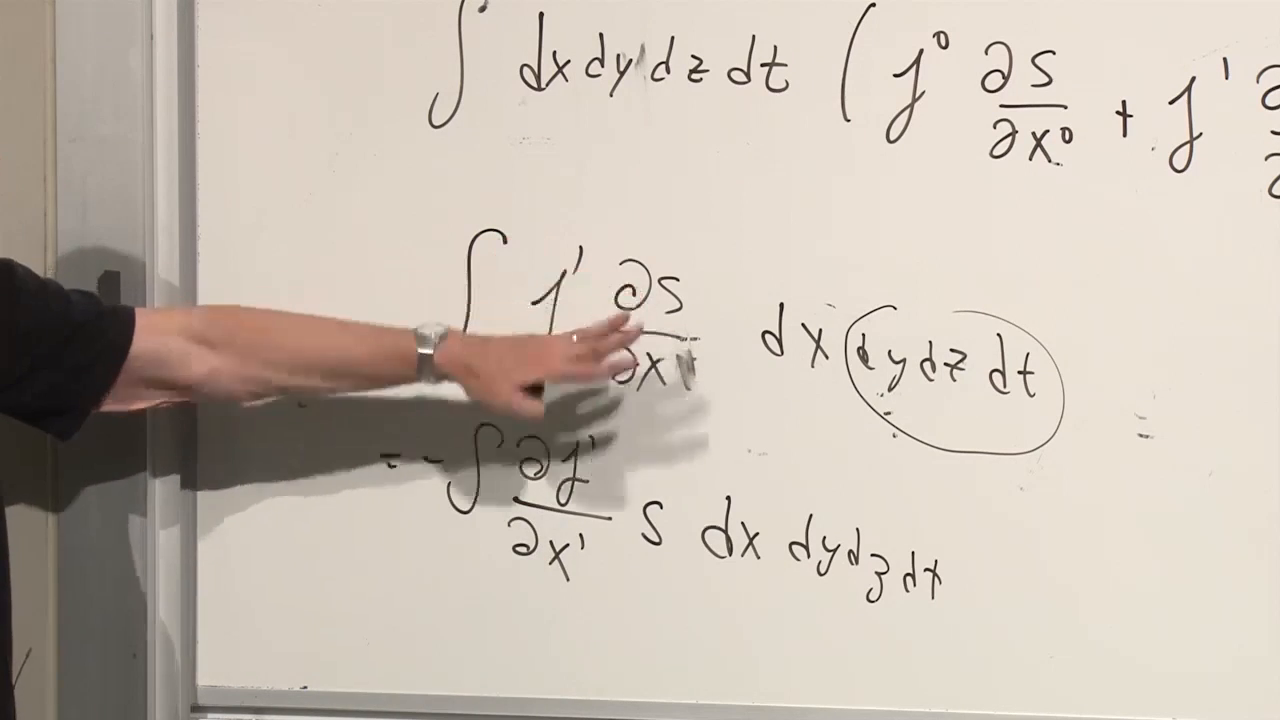
\includegraphics[width=\linewidth]{lecture_09_figure_21.png}
\caption{一个具有代表性的分部积分，把导数从规范函数移到电流上。}
\par\smallskip
\textit{讲课画面：01:20:45。}
\end{figure}

把四个分量收集起来，
\begin{equation}
\delta_\chi S_{\mathrm{int}}
=
\int d^4x\,\chi\,\partial_\mu J^\mu.
\label{eq:gauge-variation-continuity}
\end{equation}
因此，
\begin{equation}
\partial_\mu J^\mu=0
\quad\Longrightarrow\quad
\delta_\chi S_{\mathrm{int}}=0.
\end{equation}
在所假设的边界条件下，源相互作用恰好当电流局域守恒时才是规范不变的。

\begin{classroomqa}
\audiencequestion{只要求
\(\nabla\cdot\mathbf J=0\) 就够了吗？}
\lecturerresponse{不够。四项全都需要：
\[
\partial_\mu J^\mu
=
\dot\rho+\nabla\cdot\mathbf J=0.
\]
第一项是固定盒子中电荷密度的变化。当空间散度不为零时，只要它与该变化相平衡，就是允许的。\lecturetimestamp{01:22:00}}
\end{classroomqa}

\section{有源麦克斯韦方程}

完整的电磁拉格朗日密度是
\begin{equation}
\boxed{
\mathcal L
=
-\frac14F_{\mu\nu}F^{\mu\nu}
-J^\mu A_\mu.
}
\label{eq:full-maxwell-lagrangian}
\end{equation}
源项不含 \(A_\nu\) 的导数，因此它使
\eqref{eq:maxwell-canonical-derivative} 保持不变，并贡献
\begin{equation}
\frac{\partial\mathcal L}{\partial A_\nu}=-J^\nu.
\end{equation}
于是欧拉--拉格朗日方程给出
\begin{equation}
-\partial_\mu F^{\mu\nu}=-J^\nu,
\end{equation}
或者
\begin{equation}
\boxed{\partial_\mu F^{\mu\nu}=J^\nu.}
\label{eq:sourced-maxwell-from-action}
\end{equation}

\begin{figure}[H]
\centering
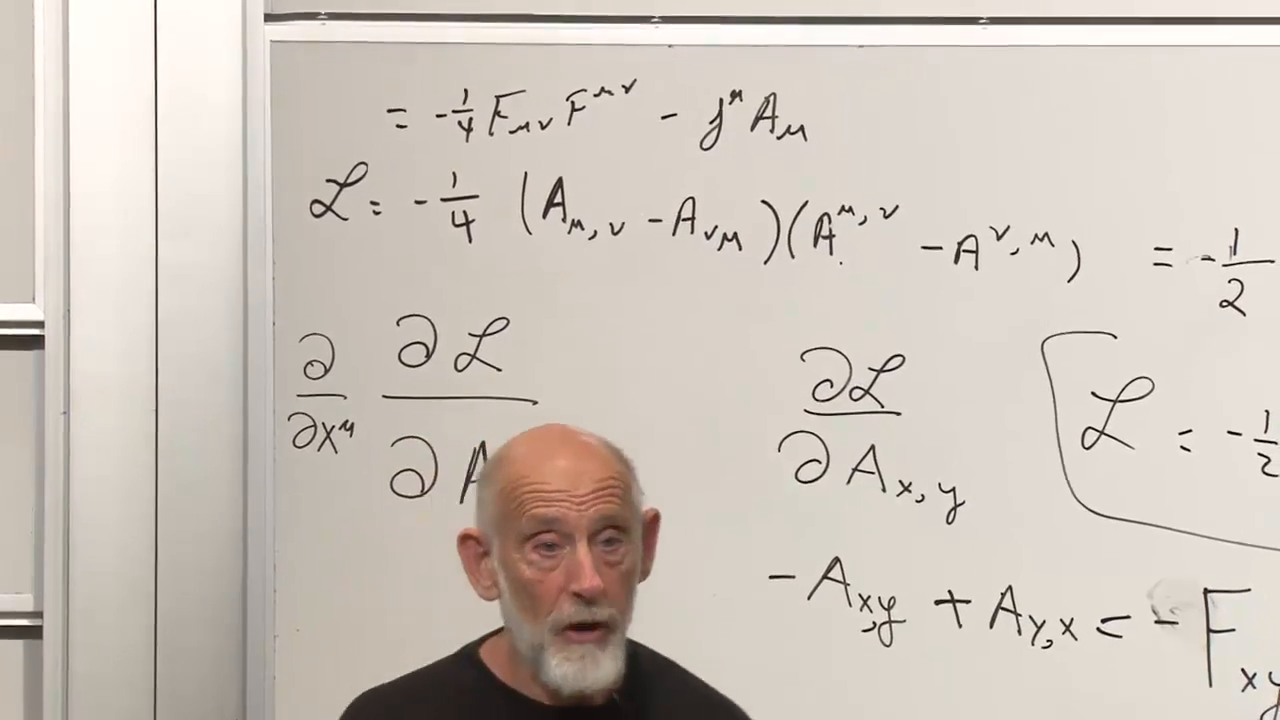
\includegraphics[width=\linewidth]{lecture_09_figure_22.png}
\caption{自由项和源项与具有代表性的欧拉--拉格朗日导数一起展示。}
\par\smallskip
\textit{讲课画面：01:25:00。}
\end{figure}

一个不守恒的给定电流会同时导致两处失败。相互作用作用量将不是规范不变的，而有源麦克斯韦方程将不自洽。电荷不能在一个区域内简单地消失，而不伴随通过其边界的补偿通量。

\section{麦克斯韦方程把守恒还了回来}

这种相容性可以直接从场方程读出。对 \eqref{eq:sourced-maxwell-from-action} 取
\(\partial_\nu\)，得到
\begin{equation}
\partial_\nu J^\nu
=
\partial_\nu\partial_\mu F^{\mu\nu}
=0,
\label{eq:antisymmetry-implies-continuity}
\end{equation}
因为导数在
\(\mu\leftrightarrow\nu\) 下是对称的，而 \(F^{\mu\nu}\) 是反对称的。

课上还用三矢量形式检验了这一点，而这一检验暴露出一个实际存在的符号错误。从高斯定律出发：
\begin{equation}
\rho=\nabla\cdot\mathbf E.
\end{equation}
对时间求导：
\begin{equation}
\dot\rho=\nabla\cdot\dot{\mathbf E}.
\label{eq:rho-dot-div-edot}
\end{equation}
黑板上暂定的方程写成了
\begin{equation}
\dot{\mathbf E}
=
-\nabla\times\mathbf B+\mathbf J.
\label{eq:provisional-wrong-source-sign}
\end{equation}
它的散度会给出
\begin{equation}
\dot\rho=\nabla\cdot\mathbf J,
\end{equation}
因为旋度的散度为零。这与
\eqref{eq:continuity-vector-l9} 矛盾。

\begin{figure}[H]
\centering
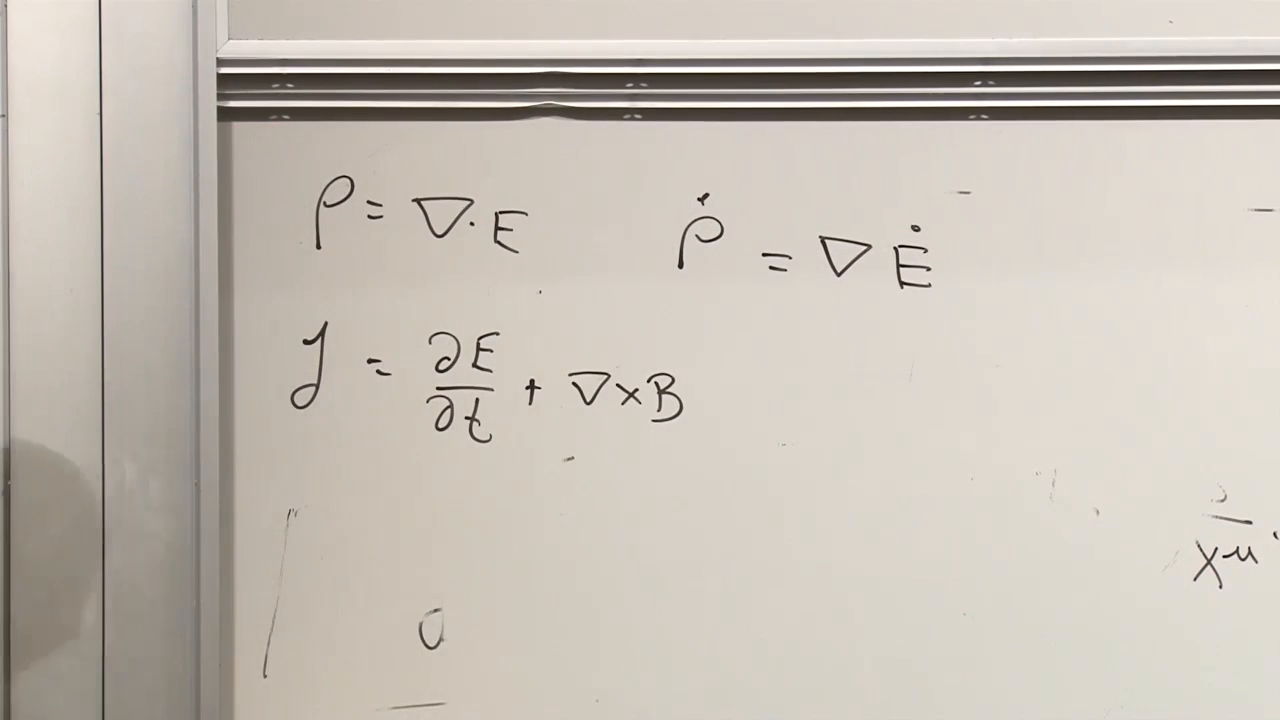
\includegraphics[width=\linewidth]{lecture_09_figure_23.png}
\caption{产生错误连续性符号的暂定带正号 \(\mathbf J\) 的黑板方程。}
\par\smallskip
\textit{讲课画面：01:27:00。}
\end{figure}

这一不匹配并没有被掩盖。计算被实时重新推演；所需的连续性方程被陈述出来；一位听众检验了方程并指出了源项的符号。按惯例自洽的分量方程是
\begin{equation}
\boxed{
\dot{\mathbf E}+\nabla\times\mathbf B=-\,\mathbf J,
}
\label{eq:corrected-source-sign}
\end{equation}
或者
\begin{equation}
\dot{\mathbf E}
=
-\nabla\times\mathbf B-\mathbf J.
\end{equation}
现在，方程 \eqref{eq:rho-dot-div-edot} 和
\eqref{eq:corrected-source-sign} 给出
\begin{align}
\dot\rho
&=
\nabla\cdot
\left(-\nabla\times\mathbf B-\mathbf J\right)
\nonumber\\
&=
-\nabla\cdot\mathbf J,
\end{align}
这恰好就是局域电荷守恒。

\begin{figure}[H]
\centering
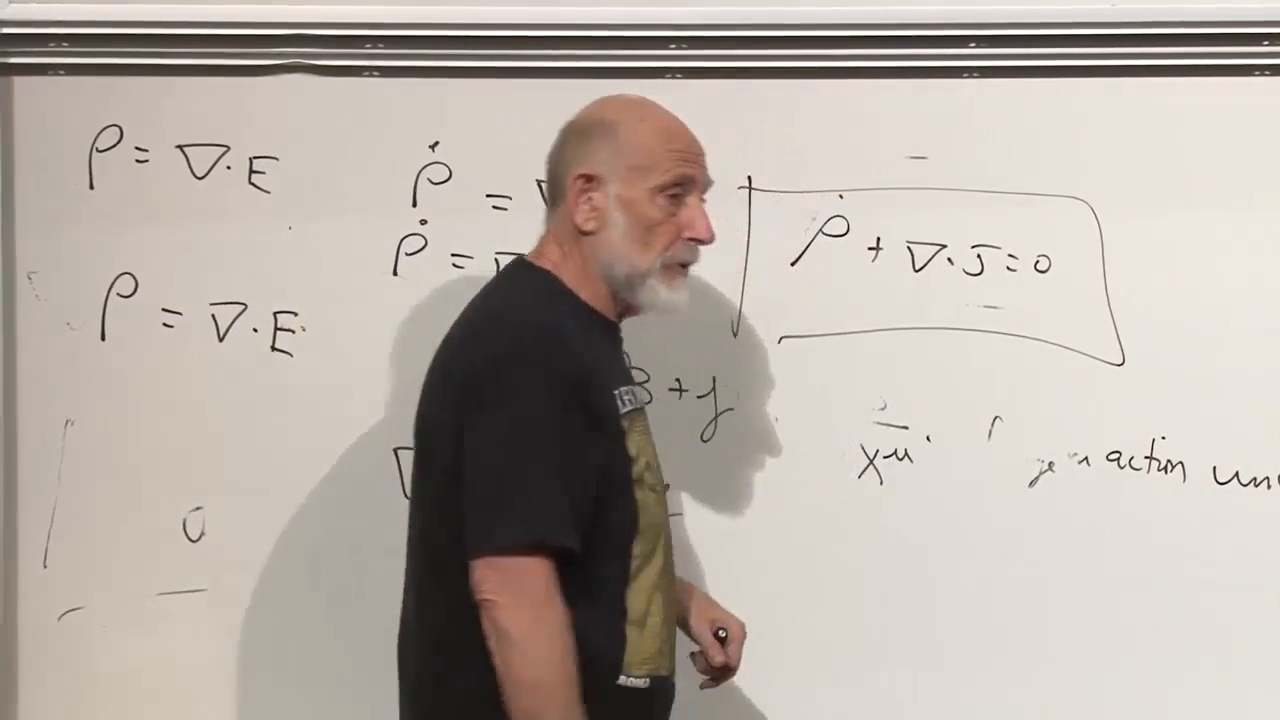
\includegraphics[width=\linewidth]{lecture_09_figure_24.png}
\caption{修正后的源符号与恢复的连续性方程。}
\par\smallskip
\textit{讲座时间轴：01:31:00。}
\end{figure}

\begin{classroomqa}
\audiencequestion{右边的电流项是否应为
\(-\mathbf J\)？}
\lecturerresponse{是的。按照本课程始终采用的场张量约定，
\(\partial_\mu F^{\mu\nu}=J^\nu\) 的空间部分为
\(\dot{\mathbf E}+\nabla\times\mathbf B=-\mathbf J\)。
这一修正使散度计算能够重现
\(\dot\rho+\nabla\cdot\mathbf J=0\)，并且不改变此前的
协变作用量推导。 \lecturetimestamp{01:30:17}}
\end{classroomqa}

\section{哪个原理是基本的？}

\begin{classroomqa}
\audiencequestion{这一推理是循环论证吗？我们用电荷守恒使作用量具有规范不变性，然后用作用量导出麦克斯韦方程组，而麦克斯韦方程组又蕴含电荷守恒。}
\lecturerresponse{这些陈述彼此相容，并不是一个预设自身结论的循环证明。人们可以从观测到的麦克斯韦方程组出发，发现连续性方程；然后认识到
\(-J^\mu A_\mu\) 是规范不变的耦合。或者，人们可以从局域性、洛伦兹不变性、规范不变性和一个作用量出发；规范不变性要求存在守恒流，而作用量给出麦克斯韦方程组。又或者，人们可以把电荷不会局域地消失这一物理事实视为首要的。每条路径都通向相同的结构。 \lecturetimestamp{01:31:11}}
\end{classroomqa}

如果问最经济的构造性路径，那么局域性、洛伦兹不变性、规范不变性与拉格朗日原理的组合会选出
\begin{equation}
-\frac14F_{\mu\nu}F^{\mu\nu}-J^\mu A_\mu
\end{equation}
并由此选出麦克斯韦动力学方程。称这个三角形中的某一项比其他项更基本，部分地取决于品味。重要的事实是这些项彼此契合。

\section{为什么用“\emph{规范}”这个词？}

\begin{classroomqa}
\audiencequestion{数学是清楚的，但
\emph{规范}这个词在这里是什么意思？}
\lecturerresponse{这个名称是一种历史性的时代错置。规范可以指选定的零点，例如相对于某个参考来测量压强。赫尔曼·外尔最初把这一想法与长度的局域标准联系起来；那种解释并不是正确的物理。当这一自由度被正确地与量子波函数的相位联系起来时，这个术语保留了下来。在当前的经典计算中，把
\(A_\mu\) 改变 \(\partial_\mu\chi\) 会改变描述性的零点，而不改变 \(F_{\mu\nu}\)。更深层的量子含义留待以后讨论。
\lecturetimestamp{01:34:49}}
\end{classroomqa}

这一历史标签不应掩盖起作用的陈述：由 \eqref{eq:gauge-transform} 联系起来的势描述同一个电磁场。因此，规范自由度是势描述的一种冗余，而场张量是规范不变的。

\section{为什么麦克斯韦方程组的两个族看起来不对称}

\begin{classroomqa}
\audiencequestion{如果电场和磁场如此对称，为什么麦克斯韦方程组的一个族表现为比安基恒等式，而另一个族来自运动方程？}
\lecturerresponse{在无源电磁学中，可以引入一个对偶势，使角色互换：原本是运动方程的东西变成比安基恒等式，反之亦然。物理上的不对称通过源进入。电荷被观测到，而基本磁单极子尚未被观测到。如果存在一个精确的普通对称性交换电荷与磁荷，人们就会期待存在具有相应谱的磁对应物，而这些并未被看到。更精致的理论仍然可以包含磁荷或电--磁对偶性，但这超出了当前的推导。 \lecturetimestamp{01:37:11}}
\end{classroomqa}

因此，无源方程具有电--磁互换结构，而观测到的源扇区选择了电的描述。这不仅仅是一种排版约定，但它并不使自由平面波中可见的对称性失效。

\section{已经组装起来的内容}

本讲所走的路线至此已经完整：
\begin{enumerate}
\item 麦克斯韦方程组迫使平面波为横波，其电场与磁场正交，且色散关系为
      \(\omega=ck\)。
\item 比安基方程是由势导出的恒等式；缩并后的方程则是动力学方程。
\item 局域性与洛伦兹不变性引导我们得到作用量密度，而规范不变性排除了 \(A_\mu A^\mu\)，并选出一个由 \(F_{\mu\nu}\) 构成的标量。
\item 自由作用量
      \(-\tfrac14F_{\mu\nu}F^{\mu\nu}\) 给出真空中的麦克斯韦方程。
\item 相互作用项 \(-J^\mu A_\mu\) 是规范不变的，当且仅当电流满足连续性方程。
\item 有源作用量给出
      \(\partial_\mu F^{\mu\nu}=J^\nu\)，而反对称性又给出
      \(\partial_\mu J^\mu=0\)。
\end{enumerate}

这已是相当庞大的结构：拉格朗日力学、相对论场论、电动力学、洛伦兹不变性、规范不变性以及局域电荷守恒，都已成为同一个论证的组成部分。要消化它，唯一可靠的办法是从方程重新开始，亲手把每一个导数和每一个符号都推导一遍。
